%% STAT 215B, Spring 2012
%% Final Project
%% Note: need to use XeLaTeX to compile

\documentclass[11pt]{article}
\usepackage[letterpaper, hmargin={1in,1in}, vmargin={1in,1in}, noheadfoot]{geometry}
\usepackage{listings} % for including source code

%\usepackage[usenames,dvipsnames]{color}

\usepackage{hyperref, graphicx}

\usepackage{amsmath}
\usepackage{amssymb}
\usepackage{ marvosym }

%%% for displaying Chinese
\usepackage{fontspec,xltxtra,xunicode}
\usepackage[slantfont,boldfont]{xeCJK}

% 设置中文字体
% ==========================================================
\setCJKmainfont[BoldFont=STHeiti]{STSong}
\setCJKsansfont{STHeiti}
\setCJKmonofont{STFangsong}
 
\setCJKfamilyfont{zhsong}{STSong}
\setCJKfamilyfont{zhhei}{STHeiti}
\setCJKfamilyfont{zhfs}{STFangsong}
\setCJKfamilyfont{zhkai}{STKaiti}
 
\newcommand*{\songti}{\CJKfamily{zhsong}} % 宋体
\newcommand*{\heiti}{\CJKfamily{zhhei}}   % 黑体
\newcommand*{\kaishu}{\CJKfamily{zhkai}}  % 楷书
\newcommand*{\fangsong}{\CJKfamily{zhfs}} % 仿宋
% ==========================================================

%%%%%%%%%%
% the following are user defined commands
\usepackage{color}
\newcommand{\note}[1]{{\em \color{red} #1}}

\newcommand{\pr}[1]{{\mathbb P}\left(#1\right)}        % probability
\newcommand{\E}[1]{{\mathbb E}\left[#1\right]}        % expectation 
\newcommand{\1}[1]{{\mathbf 1}\left\{#1\right\}}        % indicator
\newcommand{\V}[1]{\text{Var}\left(#1\right)}    % variance

\def\lp{\left(}
\def\rp{\right)}

\newtheorem{theorem}{Theorem}
\newtheorem{lemma}[theorem]{Lemma}
\newtheorem{proposition}[theorem]{Proposition}
\newtheorem{claim}[theorem]{Claim}
\newtheorem{corollary}[theorem]{Corollary}
\newtheorem{definition}[theorem]{Definition}
\newtheorem{exercise}[theorem]{Exercise}
\newtheorem{example}[theorem]{Example}

%%%%%%%%%%%
%%%%%%%%%%%

\title{\scshape Sina Weibo as a Corpus for Studying Public Opinions
	\\{\Large STAT 215B Final Project, Spring 2012} }
\author{Christine Kuang, Siqi Wu, and Angie Zhu}
\date{\today} % delete this line to display the current date

%%% BEGIN DOCUMENT
\begin{document}
\setlength\footskip{0.5in}


%%% the following is for including source code. Don't worry about it for now. --AZ
\lstset{
% backgroundcolor=\color{Gray} % requires package color
%frame=double,
showspaces=false, 
language=R, 
basicstyle=\ttfamily, 
tabsize=3, 
showstringspaces=false, 
columns=flexible%, 
%numbers=left, 
%numberstyle=\footnotesize, 
%stepnumber=5, 
%numbersep=6pt  % how far the line-numbers are from the code
}

\maketitle

%%%%%%%%%%%%%%%%%%
%%%%%%%%%%%%%%%%%%
% To Christine:
% Don't worry about the above part. The report starts from here. 
% Comments are preceded by a percentage symbol.
% LaTeX is a markup language like HTML. All the formatting is specified by particular code. 
% The structure of the report is identified by \section{}, \subsection{}, \subsubsection{}, etc. 

% I made some slides for the Productivity Seminar last Spring: http://www.stat.berkeley.edu/~luis/seminar/IntroToLaTeXSlides_Angie_Zhu.pdf
% It's very short. I have some longer intro material if you are interested.
% It covers some basic rules of LaTeX.

% I will put more reminders here for your reference :D


%% Double quotation marks: require 4 charaters ``'' (a left and a right pair of single quotes, [`] on keyboard is the one right next to [1])



%%%%%%%%%%%%%%%%%%
\begin{abstract}
{\bf Abstract.} In this project, we try to develop a framework to study the public opinions via Sina Weibo -- a Twitter equivalence in China. Text data are collected from  Weibo via an application programming interface (API). Word processing techniques are used to extract useful information from the raw data. Several standard machine learning tools are applied to feature analysis and sentiment classifications. 
\end{abstract}

%%%%%%%%%%%%%%%%%%
\section{Introduction}

Recent years have seen a growing interest of the analysis of text corpus from social media such as Facebook and Twitter. Gwalt et al (\cite{gawalt2010discovering}), for example, study word associations from a series new articles of NYTimes. Due to the increasing size of the corpus, modern sparse machine learning tools are needed in both text summarizing and topic classification. El Ghaoui et al. (\cite{ELDPSB:11}) gives an excellent summary of sparse learning tools that are useful in analyzing high dimension text data sets.  


So far most of the literatures focus on the study of English text corpus. Researches on Chinese text data have been relative few. Tan and Zhang (\cite{tan2008empirical}) conduct an empirical study of sentiment analysis in Chinese documents using a combination of feature selection methods and classification method. Lee and Renganathan (\cite{lee2011chinese}) study Chinese document via a maximum entropy method. In both of the above study, the complex structure of Chinese language makes it difficult to analyze the raw text data directly. We will explore this issue more in Section 3.1. 


Due to the restriction on overseas websites such as Facebook or Twitter, domestic substitutes have become the major platforms for the internet citizens to express their opinions towards various social or political issues. Studying posts on those website thus provides interesting insights into the public opinion. For example, some events in the recent years, such as the tragic Wenzhou train collision on July 23 2011
\footnote{For details, see \url{http://en.wikipedia.org/wiki/Wenzhou_train_collision}. }
  and the more recent Wang Lijun incident,
\footnote{For details, see \url{http://en.wikipedia.org/wiki/Wang_Lijun_incident}.}  
have split the public into two major groups among which one considers the government's way of dealing with those incidences is good and one does not. 
In principle, we can draw text data from those websites identifying whether a particular post is related to the event of interest, and which group the post should be classified into.

Sina Weibo 新浪微博 is the largest microblogging website and one of the most popular social network website in China. It had more than 300 million registered users as of February 2012 (\cite{bloombergSina})
and accounted for 65\% of China's microblog market by pageviews as of December 2011(\cite{WashingtonPostSina}).

In this project, we aim to develop a framework for studying public opinions using Sina Weibo as a corpus for a given topic. Posts are sampled from Weibo and then processed taking the characteristics of both Chinese language and Weibo posts into consideration. Two unsupervised learning tools, the sparse Gaussian graphical model and the sparse PCA are used in feature analysis. Also, the LASSO and the $l_1$-norm SVM are used in classification. 


%%%%%%%
\section{Data Collection}\label{subsec:datacol}

A Weibo  application programming interface (API) is set up to collect posts.
For a given topic, the ideal way to collect sample post are taking a random sample. \cite{boyd2004fastest, leskovec2006sampling, wang2011understanding} have presented sampling algorithms from large graphs. However, our preliminary results show that the sample contains a large proportion of spams and posts which do not relate to the chosen topic. Therefore, the topic searching functionality of the Weibo API is utilized to collect posts. 

There are certain technical restrictions on API. Regarding topical searches, only the latest search results are returned. The maximum number of posts returned is 30 and our own searches typically returned about 18 posts. There is waiting time between consecutive searches. Overlapping among sets of search results is examined. Clearly the sample is time-sensitive. We preferred having a relatively short collection time so as to obtain a cross-sectional sample. Hence, the chosen topic for testing should have active discussion on Weibo. 

It is well-known that China has strict Internet censorship compared to other countries. Even though the downfall of Bo Xilai
\footnote{For more information on Bo Xilai, see \url{http://en.wikipedia.org/wiki/Bo_Xilai}.}
was a hot topic at the time of our data collection, there were no meaningful posts on Weibo. 
The topic we finally chose is Han Han 韩寒. 
\footnote{For more information on Han Han, see \url{http://en.wikipedia.org/wiki/Han_Han} and {\em Han Han: China's Literary Bad Boy} by Simon Elegant Monday, published on November 02, 2009, {em Time Magazine}, \url{http://www.time.com/time/magazine/article/0,9171,1931619,00.html}.}
Born September 23, 1982, Han Han
is a Chinese best-selling author, professional rally driver, and  wildly  popular blogger. He published his first novel {\em Triple Gate 三重门} at the age of 17 and later dropped out of high school. Even though Han Han is famous for his criticism on social issues, he has not been heavily censored. A ghostwriting allegation against Han Han started in January 2012. Fang Zhouzi 方舟子,
\footnote{For more information on Fang Zhouzi, see \url{http://en.wikipedia.org/wiki/Fang_Zhouzi}.}
 a scientific author and anti-fraud crusader, created widespread debate with Han Han on the Internet regarding the ghostwriting allegation. In response to the allegation, Han Han published a photocopied manuscripts set {\em Light and Upright 光明与磊落} in April 2012, including the manuscript of his first novel {\em Triple Gate}. 
 
Han Han received an online death threat on April 15, 2012. We collected a set of 22,398 posts on April 16 and 17, 2012. The above proper nouns and words related to the death threat appeared frequently in our data set. 




%%%%%%%
\section{Processing}

%%%

\subsubsection{Encoding}
Chinese documents use various encoding standards (\cite{wong2009introduction}). {\em GB 国标}, abbreviation for ``National Standard'' in Chinese, is the standard used in mainland China, Singapore, and Malaysia. Since GB is unable to cover traiditional Chinese characters, {\em GBK 国标扩展}, ``Extension of National Standard,'' is developed to support both simplified and traditional characters. Meanwhile, {\em Big5} is the encoding standard used by Taiwan, Hong Kong, and Macau. {\em Unicode} is an industry standard for the consistent encoding of text expressed in most of the world's writing systems. {\em UTF-8} is the most commonly used encoding implementation of Unicode. All our data and related files use UTF-8 encoding for processing purpose.

%%
\subsection{Characteristics of Chinese Language}\label{subsubsec:Chinese}

There has been quite a bit of research done on natural language processing in the English language, but not much on the Chinese language.  This is due to the fact that the Chinese language contains unique characteristics that makes it difficult to do natural language processing on it well. 
 
First, the Chinese language, unlike the English language, has no explicit delimiter between words. In the English language, spaces separate words and so to segment a sentence into its appropriate components is not too difficult since one could just separate based on spaces.  The Chinese language however has no such delimiter between words.
 
An additional difficulty in segmenting a sentence into its appropriate components and words is that the Chinese language is made of separate characters where each character has a meaning of its own, but if you combine two or more characters together into a phrase, the meaning can be completely different. These types of ambiguities are typically easily resolved by humans reading the sentence and realizing what would make most sense in terms of the context of the
sentence, but it is not so easy for a computer to perform those types of automatic word/phrase segmentations. For example, 他好吃 -- this sentence could be separated in two ways. The first character means ``he.'' The other two words can be taken as two different phrases: ``tastes delicious'' or ``loves to eat.''  It is obvious that the phrase should be taken as "he loves to eat" because ``he tastes delicious'' does not make sense but it is difficult to have a computer
automatically recognize which sentence makes more sense. Some words also have more than one meaning. For example, 打 can be used in different ways with different meanings. It can be used in the contexts of playing a sport, hitting a person or object, or playing a game. 

Second, the Chinese language has many out-of-vocabulary (OOV) words .  These are new phrases that are not found in dictionaries.  These phrases typically result from cultural references, current hot topics, acronyms, abbreviations, names/nicknames, or informal and slang words.  Specifically to the posts that we looked into, out of vocabulary words typically occurred in the case of cultural references.  Many of these social media posts would contain nicknames created for some hot topic issue, person, or event of the week or simply popular slang or informal words and phrases used to convey an emotion.  Since social media posts are more popular with the young adult generation, many of the words used in the posts are popular informal phrases that would not normally be found in established dictionaries. Knowledge of these types of OOV words comes out of knowing the current trends in Asian countries and being up to date with the typical language used by the younger generation.  

Third, the Chinese language has two forms - traditional and simplified and it is not a one to one correspondence between the two forms which makes it difficult to convert between the two for translation or natural language processing. 


\begin{center}
\begin{figure}[!h]
   \centering
   
\includegraphics[width=0.9\textwidth]{./slides/weiboEg.png} 
      \caption{An example of Weibo posting. The picture showed Han Han met with Ma Ying-jeou, the President of the Republic of China (Taiwan), on May 3, 2012.}
   \label{fig:weiboex}
\end{figure}
\end{center}

%%
\subsection{Characteristics of Sina Weibo Posts}\label{subsubsec:Weibo}

Our analysis takes not only the characteristics of Chinese language into consideration, but also the characteristics of Sina Weibo posts.
The writing style of Weibo posts are generally informal. The users may not use standard punctuation marks for separation of sentences and parts of sentences. The most important features are described as follows:
\begin{description}
\item[Multiple Forms] A post can be text, picture, and/or multimedia as shown in Figure~\ref{fig:weiboex}. Weibo API is only able to return posts in text. For instance, we record a post in the following format:
\begin{quote}
1714080953 2012-04-16 10:01:59 //@風笑巨石: 那尊神容不得别人质疑?//@伯林2011: 
质疑派人士遭到人肉,人身攻击,甚至死亡威胁的时候,从来没有污名化整个挺韩派,也没有引起什么媒体关注,相比之下,韩寒如此炒作,太无良了,挺韩和批韩的双方本不至于如此撕裂
\end{quote}
The post starts with the user identification number and time stamp. We ignore pictures and videos at this stage. 

\item[Reposting] A user may repost another post. Reposting does not automatically imply agreement or liking. This type of post usually consists of two parts: the reposting user's comment and the post being reposted. The reposting user's comment may be empty or set as the default text ``Repost'' or ``转发微博'' (``Repost Weibo''). The reposted post itself may include multiple repostings. The reposting part usually starts with  ``//\MVAt'' followed by a user name as demonstrated in the above example and Figure~\ref{fig:weiboex}. The issue of keeping track of repostings and identifying agreements or disagreements to the topic reposted about can be a project in itself. In our analysis, only the reposting user's comment is kept for the sake of simplicity and time.  

\item[Spams] There are a fair amount of spams on Weibo. Some spam posts are identical except for the URL. Hence, URLs are first removed and then we check for duplicated posts in the pre-tagging processing step.

\item[Mentioning] A user may mention other users in their post by inserting their usernames preceded by the \MVAt\  symbol. The mentioned usernames may be integrated into the post. We define a set of topic-related usernames and substitute the mentioning of these usernames by the corresponding proper nouns. The other mentioned usernames are removed.

\item[Emotion Symbols] Sina Weibo provides users a set of emotion symbols which are denoted with a phrase indicating its corresponding meaning surrounded by square brackets. The users may use other emotion symbols, such as ``:)'' for a smile and ``T\_T'' for a crying face. 
The two classes of graphic characters in CJK (Chinese, Japanese and Korean) computing,
\footnote{For more details, see \url{http://en.wikipedia.org/wiki/Halfwidth_and_fullwidth_forms}.}
 namely fullwidth and halfwidth, make emotion symbols more complicated. The punctuation marks in the emotion symbols can be in either fullwidth or halfwidth, such as fullwidth ``。'' and halfwidth ``.'' for period. Thus, there are various combinations, even for a limited set of commonly used emotion symbols. A dictionary for emotion symbols is constructed manually by the authors.
 
\item[Internet Slangs] 
Internet slangs are a large part of Out-of-Vocabulary (OOV) words. Some substitute the characters in a word with characters that have similar pronunciations, such as ``蜀黍'' (Shu3 Shu2) for ``叔叔'' (Shu1 Shu1, means ``uncle'') and ``围脖'' (wei2 bo2, means ``scarf'') for ``微博'' Weibo (wei1 bo2). Some are popular Internet interjections, such as ``喵了个咪'' (喵: ``meow,'' 了: past tense marker, 个: universal measure word, 咪: ``mew'') which means ``dog my cats.'' Again, a dictionary for commonly used Internet slangs is constructed manually by the authors.


\item[Topic] Since the Chinese language has no explicit delimiter between words, topic words are surrounded by the pound signs {\ttfamily \#} . The topic words can be integrated into the post. 

\end{description}

 




%%
\subsection{Pre-tagging Processing}

Our data set contains 22,398 posts. 
%In order to obtain labeled messages for training and testing purpose, the authors manually provided tags to a set of randomly selected 3500 posts, among which 3000 are used for training and 500 for testing. The four types of tags used here are positive, negative, noninformative.
Due to the fair amount of spam posts and the issue of tracking down repostings described in Section~\ref{subsubsec:Weibo}, the data need to be cleaned before the constructing of the training and testing sets.
A typical post looks like:
\begin{quote}
1165303315 2012-04-16 09:55:40  《韩寒收到网友死亡威胁》 (来自 @新浪娱乐) \\ 
http://t.cn/zOprKap

1165303315 2012-04-16 09:55:40  《Han Han received death threat online》 (from @新浪娱乐) http://t.cn/zOprKap
\end{quote} 
The pre-tagging processing consists of the following steps:
\begin{enumerate}
\item The user identification number and time stamp are removed.
\item Only the reposting user's comment is kept. The reposted part is removed from further analysis. If the resulting string is empty, it will be eliminated as well.
\item URLs are removed.
\item Duplicates are removed.
\end{enumerate}

The resulting file consists of 13,070 unique posts. A set of randomly selected 3500 posts, among which 3000 are for training and 500 for testing, will be manually tagged.



%%%%%%%
\subsection{Tagging}

%Tagging Limitations

In all, we tagged a total of 3500 Weibo posts.  We made a search for the topic we were looking into and did this over time to get a total of 22,398 Weibo posts, with 13,070 posts left after pre-processing, from which we randomly picked out 3000 posts as our training set.  We split up the posts to tag by hand.  The final 500 posts were for our test set. We had a total of four different categories that we tagged the posts as -- neutral/unidentifiable, positive, negative, and irrelevant (spam).  

As we each tagged the posts, we encountered and realized some of the limitations involved. One limitation was in the fact that tagging these posts produced subjective responses.  What one of us read as a negative response to the topic we chose, another may have read as a positive response.  For example, the English phrase ``that wasn't too bad'' could be taken as positive or negative.  Positive -- the experience was better than expected; negative -- the experience wasn't great. Hence, it is difficult sometimes to truly know whether the original author of the post had in mind a negative or positive reaction to the topic he was posting about.  

Another limitation was that some posts we were not sure how to tag. Many posts consisted of just a quote by the author we were looking into.  These could have been seen as positive posts since the writer may have liked the quote and so posted it. But at the same time, the author could have been neutral and was just merely using the quote to apply to a specific circumstance in his life at the time. We were not entirely sure of how to tag each of the posts that fell into this category, and so again, the subjectiveness of tagging the posts by hand comes into play as a limitation in the forming of our model.  Another uncertainty that occurred in trying to manually tag the posts was that some of the posts didn't talk about our chosen topic specifically, but a related topic.  With our chosen topic, people who had negative responses towards 韓寒 (Hanhan), were usually on the side of the opposing author who was discrediting him.  Some of the posts did not directly mention 韓寒, but would instead show support for the opposing side. With these posts, we typically labeled as a negative response.  However, an argument could be made for just throwing out those posts since they do not directly say anything about 韓寒, and they could possibly just be supporting the opposing author in his own literary works and not necessarily in his stance against 韓寒.  Another uncertainty in tagging is what to tag posts that have no subject.  There were a few posts that had nothing to do with the chosen topic at all, but there were also posts that had no subject but contained phrases such as ``Keep it up!'' and ``always a supporter!'' that could very well be taken as positive posts since our search is for our specific topic. But because there is no subject in the posts, this cannot be taken with 100\% certainty. In these instances, where there is no subject in the posts, we marked them as irrelevant to be on the conservative side in our predictions. 

These limitations in tagging will affect our model's accuracy in predicting whether a post contains a positive or negative response to the topic at hand.  These limitations also indicate to us that in general, models for predicting whether or not a social media post is negative or positive towards a chosen topic is limited greatly by the subjectiveness of the sentence's meaning and interpretation which affects the training set used to form the model. This limitation could present a potential future question to look into on how we can improve tagging -- whether we should just remove posts that have too subjective of an interpretation to tag or if by studying these types of ambiguous posts, we can create certain priors or statistical models to help in the tagging process. 



%%
\subsection{Pre-segmentation Processing}

As discussed in Section~\ref{subsubsec:Chinese}, sentences in Chinese are normally strings of Chinese characters without spaces between words. Hence, word segmentation is crucial for our word-based analysis. According to the characteristics of Weibo posts described in Setion~\ref{subsubsec:Weibo}, the following processing steps are preformed:
\begin{enumerate}
\item A set of topic-related usernames are defined.  Any mentioning of these usernames are substituted by the corresponding proper nouns. The other mentioned usernames are removed.
\item A set of emotional symbols and Internet slangs are defined.  They are then substituted by the corresponding word surrounded by square brackets.
\end{enumerate}

	

%%
\subsection{Segmentation}

汉语词法分析系统ICTCLAS (Institute of Computing Technology, Chinese Lexical Analysis System) is a well known Chinese word segmentation system developed by 
%Institute of Computing Technology, Chinese Academy of Sciences 
\\ \cite{ICTCLAS}. It offers the functionality of  Chinese word segmentation, lexical tagging, named entity recognition, unknown words detection, and the user-defined dictionary. 
The current version is ICTCLAS 2011, which supports GB2312, GBK, UTF8 and several encodings and has a precision rate of 98.45\%. 

The Java version of ICTCLAS 2011 performs word segmentation and lexical tagging on a Linux 32-bit machine. A user-defined dictionary is provided. The entries in this dictionary contain proper nouns and Internet specific words. For instance, some users refer to Han Han as 韩少 (韩: Han Han's surname, 少: abbreviation of 少爷, which means ``young master of the house''). 
Even with the user-defined dictionary, some appearances of Han Han's name 韩寒 can not be segmented and tagged correctly. Hence we account and correct for this directly using regular expression.

%%	
\subsection{Conjunction Rules}

%Lee and Renganathan 
\cite{lee2011chinese} noted that special consideration should be given to the sentences whose parts are linked by contrasting transitional expressions. In particular, if a sentence contains conjunctions such as ``although'' and  ``but,'' only the part being emphasized will be kept and used to infer the sentiment polarity of the sentence. We considered these three cases:
\begin{enumerate}
\item Although (part A), (part B).
\item (Part A), but (part B).
\item Although (part A), but (part B).
\end{enumerate}
For each case, only part B will be kept. 

The four words for ``although'' are 虽然, 虽说, 虽, and 尽管. The words for ``but'' are 但, 但是, 不过, 可是, 然而, 只是, 可, 只, 然, and 却. 



%%
\subsection{Stop Words and Punctuation Elimination}
Moreover, stop words, non-text strings, and punctuation marks are eliminated based upon the lexical tags generated by ICTCLAS. The detailed process is as follows: 
\begin{enumerate}
\item  Remove prepositions, punctuation marks, English character strings, interjections, modal particles, onomatopoeia, and auxiliary words.
\item Remove pre-defined stop words and number strings.
\end{enumerate}
Note that the pre-defined stop words do not contain the following six negation words:  不, 不是, 没有, 没, 无, and 别. These negation words will be used in sentiment score assignment.


%%%%%%%
\begin{center}
\begin{figure}[tb]
   \centering
   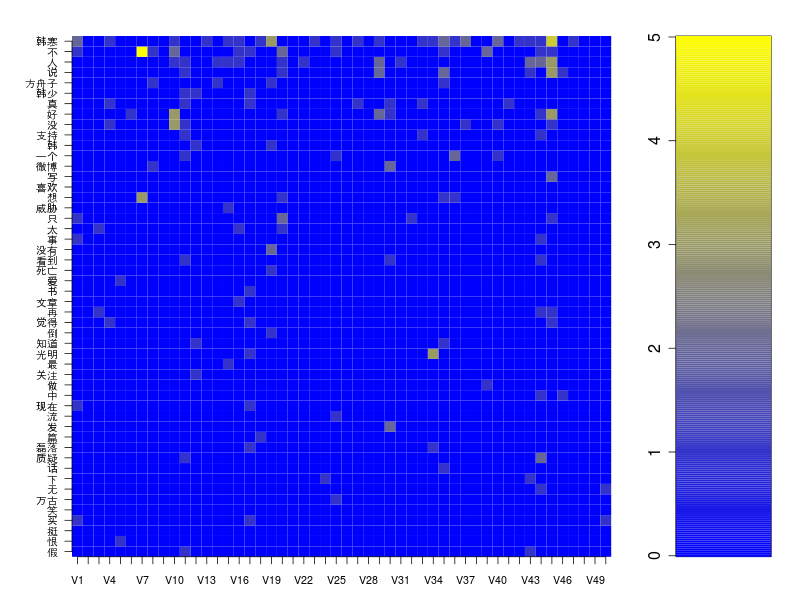
\includegraphics[width=\textwidth]{../wordFreqMat.png} 
      \caption{Plot of the transpose of the frequency matrix.}
   \label{fig:freqmat}
\end{figure}
\end{center}


\section{Feature Analysis}
It is of interest to study the relation between words or phrases in the posts. In what follows, we will base our analysis on the frequency matrix $X\in R^{n\times p}$, where the entry $x_{ij}$ stores the frequency of occurrences of the $j$-th word(or phrase) in the $i$-th post. We include only words or phrases that have total occurrence of at least 10 times over all 3000 posts. Analyzing feature relations can help us better understand word usage and identify possible clusters in the feature space.  Figure~\ref{fig:freqmat} shows the frequency of the top 50 most frequent words in the first 50 posts.


One possible way to visualize word usage relation is to look at the concurrence between any two pair of words. Denote by $C$ the concurrence matrix, where the entry $c_{ij}$ records the number of concurrencies of the $i$-th and the $j$-th word in the same post. Figure~\ref{fig:coocurmat} and \ref{fig:coocur} give the matrix plot and the network plot of the top 50 most frequent words. 


%%
%\note{ 
%To Christine: in the notes below the frequency matrix, comment on the sparsity of the data. then point out the need to use high dimension tools in the later-on section.
%}

As can be seen from Figure~\ref{fig:freqmat}, our data is quite sparse; most words do not appear too many times in each post. 
Due to the sparseness of our data, we chose methods of modeling our data accordingly (as will be described
in further detail in later sections). We use high dimensional tools to take into account the sparseness of our 
frequency matrix.  This frequency matrix will be our design matrix for our models.  




\begin{center}
\begin{figure}[tb]
   \centering
   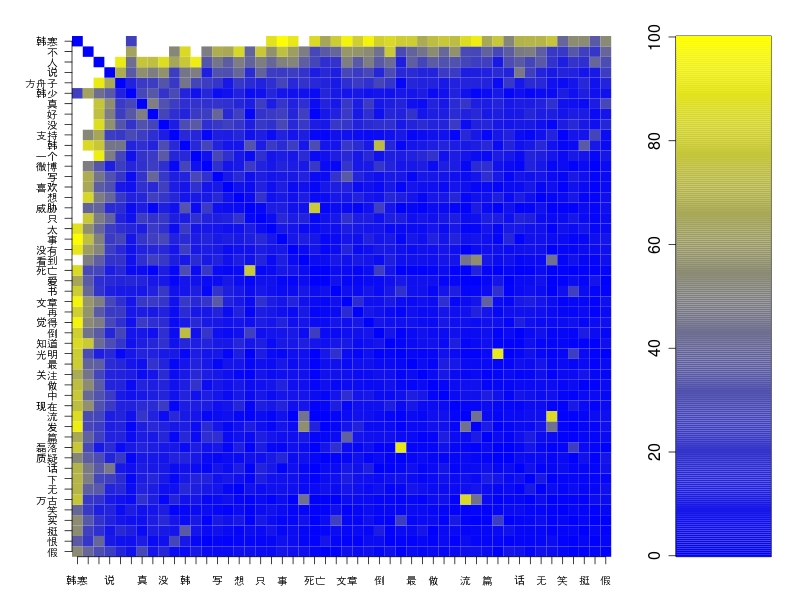
\includegraphics[width=\textwidth]{../coocurResults/cooccurMatPlot.png} 
      \caption{Plot of the word concurrence matrix $C$. Only top 50 most frequent words are shown.}
   \label{fig:coocurmat}
\end{figure}
\end{center}

\begin{center}
\begin{figure}[tb]
   \centering
   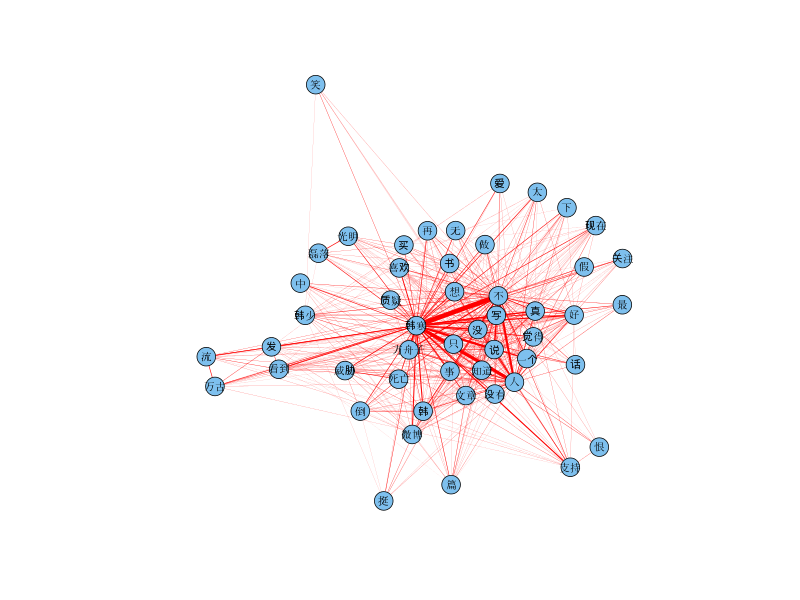
\includegraphics[width=\textwidth]{../coocurResults/cooccurNetwork.png} 
      \caption{Network plot of the word concurrence matrix $C$. Only top 50 most frequent phrases are shown.}
   \label{fig:coocur}
\end{figure}
\end{center}



%%%%%%%%%%%%%%%%%%%%%%%%%%%%%%%%%%
\subsection{Sparse Principal Component Analysis (SPCA)}
Principal component analysis (PCA) is a standard approach for feature extraction and dimension reduction. In high dimensional settings, \cite{zou2006sparse} suggest the following variant of the traditional PCA:
\begin{align*}
(A,B) & = \arg \min_{A,B} \left \{ \sum_{i=1}^n||x_i-AB^Tx_i||_2^2 + \sum_{j=1}^k\lambda_{j}||\beta_j||_1 \right\} \\ 
\text{subject to } & A^TA = I_{k}. \nonumber
\end{align}
In the above formulation, only the first $k$ leading principal components are kept, with the corresponding loading matrix $B = (\beta_1,...,\beta_k) \in R^{p\times k}$. The feature vector $x_i$'s are required to be demeaned. Different regularization parameters $\lambda_{j}$ are used for the $l_1$ norm of the loadings. To solve the SPCA problem, we use the efficient algorithm proposed by \cite{zou2006sparse}. 

%(A,B) & = \arg \min_{A,B} \left \{ \sum_{i=1}^n||x_i-AB^Tx_i||_2^2 + \lambda \sum_{j=1}^k||\beta_j||^2 + \sum_{j=1}^k\lambda_{1,j}||\beta_j||_1 \right\} \\ 
%\text{subject to } & A^TA = I_{k}. \nonumber
%\end{align}
%In the above formulation, only the first $k$ leading principal components are kept, with the corresponding loading matrix $B = (\beta_1,...,\beta_k) \in R^{p\times k}$. The feature vector $x_i$'s are required to be demeaned. The same $\lambda$ is used to penalized the square $l_2$ norm of all the loading coefficients whereas different regularization parameters $\lambda_{1,j}$ are used for the $l_1$ norm of the loadings. To solve the SPCA problem, we use the efficient algorithm proposed by \cite{zou2006sparse}. 

%By doing a sparse PCA on the frequency matrix, we hope to find possible principal components that can summarize the 3000 posts we targeted. For simplicity, we set the number of principal components $k=3$ and tune for the regularization parameters. The results are summarized in Table~\ref{tb:spca}.

By doing a sparse PCA on the frequency matrix, we hope to find possible principal components that can summarized the 3000 posts in the training set. For simplicity, we set the number of principal components $k=3$ and tune for the regularization parameters. The words with top loading coefficient in each of the three principal components are listed in Table~\ref{tb:spca}.

\begin{table}[htb]
\caption{Sparse PCA results on the frequency matrix ($\lambda_1=\lambda_2=\lambda_3 = 10$).}
\begin{center}
\begin{tabular}{|c|c|c|}
\hline
1st PC top abs.coef.  &  2nd PC top abs.coef   & 3rd PC top abs.coef \\ \hline
     韩寒 (Han Han)      &       方舟子 (Fang Zhouzi)    &   死亡 (death)\\ \hline
     韩少 (Master Han)   &        够 (enough)        &        韩 (Han)\\ \hline
     写 (write)         &       质疑 (suspect)        &     威胁 (Threat)\\ \hline
     真 (truth)         &         韩 (Han)         &         倒 (oppose)\\ \hline
     死亡 (death)         &       事 (event)      &         网友 (netizen)\\ \hline
\end{tabular}
\end{center}
\label{tb:spca}
\end{table}%

It is surprising how the above results from sparse PCA are related to our prior knowledge of the subject. The first principal seems to be about the Han Han the person and perhaps his writing; the second column is related to the fact that the fraud-crusader Fang Zhouzi suspects the authorship of HanHan's works; the third is about the death threat to Han Han. Thus all these three components seem to correspond to the three major aspects of Han Han that are known to us prior to our analysis. See Section~\ref{subsec:datacol} again.


%It is easy to see that the first principal seems to be about the writing of Han Han; the second principal is related to the fact that the fraud-crusader Fang Zhouzi suspects the authorship of HanHan's works; the third is about the death threat to Han Han. These three components correspond to three major aspects of Han Han that are known to us as discussed in Section~\ref{subsec:datacol}.


%%%%%%%%%%%%%%%%%%%%%%%%%%%%%%%%%%%
\subsection{Sparse Graphical Models}
%Graphical models are commonly used in machine learning to study the relation between random variables (\cite{wainwright2008graphical}). Here we consider undirected graphical representations of random variables. Each node of the graph represents a random variable. An edge connecting two nodes represents the conditional dependency between the two random variables given all other random variables (the absence of an edge indicates conditional independency). If, in addition, the joint distribution of the random variables is a multivariate normal with mean $\mu$ and covariance matrix $\Sigma$, then the $i$-th node and $j$-th node are conditionally independent (or, equivalently, missing an edge) if and only if $(\Sigma^{-1})_{ij} = 0$. Therefore, given data $x_1,x_2,...,x_n\in R^p$, to explore the relation between features, we can estimate the inverse covariance matrix by computing the MLE:   

Undirected graphical models are commonly used in machine learning to study the relation between random variables (\cite{wainwright2008graphical}). Each node of the graph represents a random variable and an edge connecting two nodes represents the conditional dependency between the two random variables given all other random variables (and the missing of an edge indicates conditional independency). If, in addition, the joint distribution of the random variables is a multivariate normal with mean $\mu$ and covariance matrix $\Sigma$, then the $i$-th node and $j$-th node are conditionally independent (or, equivalently, missing an edge) if and only if $(\Sigma^{-1})_{ij} = 0$. Therefore, given data $x_1,x_2,...,x_n\in R^p$, to explore the relation between features, we can estimate the inverse covariance matrix by computing the MLE:   

\begin{align}
\label{eq:mle}
\max_S \left\{  \log \det \lp S\rp - \textbf{Tr}( \hat{\Sigma}S)  \right\}
\end{align}
If the number of features $p$ is large, certain regularization is needed to control the number of edges. Banerjee et al. (\cite{banerjee2008model}) propose the following optimization problem to recover the sparse structure in a gaussian graphical model
\begin{align}
\label{eq:gLasso}
\max_S \left\{ \log \det S - \textbf{Tr} \lp \hat{\Sigma}S \rp - \lambda ||S||_1 \right\}
\end{align}
%where $\Sigma$ is the covariance matrix of the data/design matrix $X$ and $||S||_1 = \sum_{i=1}\sum_{j=1} |s_{ij}|$. To solve for $S$,  Banerjee et al. (\cite{banerjee2008model}) propose a block coordinate ascent method (COVSEL) (updating one row and one column of $S$ at one time). Their approach is exact but also time consuming. Meinshausen and Buhlmann (\cite{meinshausen2006high}) use an approximation approach that is substantially faster. In our study, we adopt the fast and accurate graphical LASSO procedure ({\sffamily R} package {\sffamily glasso}, \cite{Rglasso}). Figure~\ref{fig:glasso1} shows the word usage network by fitting a sparse graphical model. Due to space limit, only the top 50 most frequent words are shown.

where $||S||_1 = \sum_{i=1}\sum_{j=1} |s_{ij}|$. To solve for $S$,  Banerjee et al. (\cite{banerjee2008model}) propose a block coordinate ascent method (updating one row and one column of $S$ at one time). Their approach is exact but is time consuming. Meinshausen and Buhlmann (\cite{meinshausen2006high}) uses an approximation approach that is substantially faster. In our study, we adopt the fast and accurate graphical LASSO procedure ({\sffamily R} package {\sffamily glasso}, \cite{Rglasso}). Figure~\ref{fig:glasso1} shows the word usage network by fitting a sparse graphical model for $\lambda=0.01$. Different values of the regularization parameters are tuned and more such plots can be found in Appendix A. 


%\note{lambda = 0.01 plot here.}

\begin{center}
\begin{figure}[tb]
   \centering
   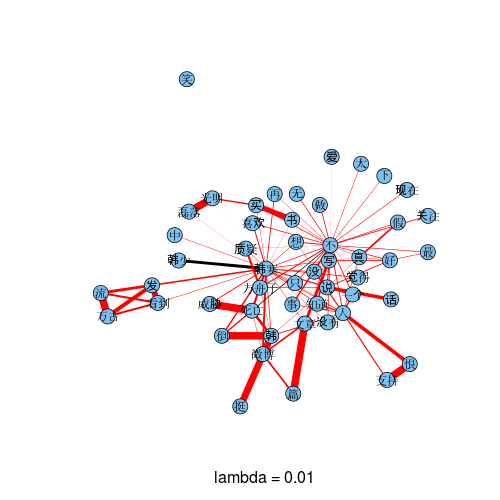
\includegraphics[width=0.7\textwidth]{../gLassoResults/glasso1.png} 
      \caption{The network plot of the estimated inverse covariance matrix $S$, with $\lambda = 0.01$. As discussed, an edge (i.e. $S_{ij}\neq 0$) represents conditional dependency between two nodes given all the other nodes. Red edges indicate positive correlated occurence $S_{ij}<0$ (Given all other words, word $i$ is more likely to occur if word $j$ is observed) and black edges indicate negative correlated occurrence $S_{ij}>0$. Edge width is proportional to $|S_{ij}|$, representing the strength of the tie. Again, due to space limit, only the top 50 most frequent words are shown.}
   \label{fig:glasso1}
\end{figure}
\end{center}

We can make a comparison between the concurrence network (Figure~\ref{fig:coocur}) and sparse graphical model (Figure~\ref{fig:glasso1}): the concurrence network is heavily influenced by usage frequency of words. For example, ``不'' (the negation word) and ``韩寒''(Han Han) are strongly connected in the concurrence network, but this might not imply that there is an nontrivial relation between these two words. Sparse graphical models, on the other hand, give more interpretable results. For example,  ``不''(the negation word) and ``韩寒''(Han Han) are not longer heavily connected. In addition, some interesting word combinations are revealed: the word ``光明'' (light) and ``磊落'' (upright) are words that constitute the name of the Han Han's new book {Light and Upright} as mentioned in Section~\ref{subsec:datacol}; and the clique form by ``方舟子'' (Fang Zhouzi),''怀疑'' (suspect) and  ``韩寒'' (Han Han) seems to reveal the fact that Fang suspects Han Han has a team of ghost writers. Other obvious relation revealed include ``死亡'' (death) and ``威胁'' (threat), ``买'' (buy) and ``书'' (book), ``写'' (write) and ``文章'' (article),  and so forth.

It is also of interest to observe how the word usage network structure change as we change the regularization parameter $\lambda$. From Figure~\ref{fig:glasso1}-~\ref{fig:glasso6} in Appendix A one can see that widths of the edges weaken and the number of edges decreases. Only strong conditional dependency between two words can survive for the largest regularization parameter we try: $\lambda = 0.03$, e.g. word pairs like ``死亡'' (death) and ``威胁'' (threat), and ``方舟子'' (Fang Zhouzi) and ``韩寒'' (Han Han).  


%The network plot of the estimated inverse covariance matrix $S$ is shown. As discussed, an edge (i.e. $S_{ij}\neq 0$) represents conditional dependency between two nodes given all the other nodes. Red edges indicate positive correlated occurence $S_{ij}<0$ (Given all other words, word $i$ is more likely to occur if word $j$ is observed) and black edges indicate negative correlated occurrence $S_{ij}>0$. Edge width is proportional to $|S_{ij}|$, representing the strength of the tie.


%A comparison of the concurrence network (Figure~\ref{fig:coocur}) and sparse graphical model (Figure~\ref{fig:glasso1}): the concurrence network is heavily influenced by usage frequency of words. For example, ``不'' (the negation word) and ``韩寒''(Han Han) are strongly connected in the concurrence network, but this might not imply that there is a nontrivial relation between these two words. Sparse graphical models, on the other hand, give more interpretable results. For example,  ``不''(the negation word) and ``韩寒''(Han Han) are no longer heavily connected. In addition, some interesting word combinations are revealed: the word ``光明'' (light) and ``磊落'' (upright) are words that constitute the name of the Han Han's new book {Light and Upright} as mentioned in Section~\ref{subsec:datacol}; and the phrase formed by ``方舟子'' (Fang Zhouzi),''怀疑'' (suspect) and  ``韩寒'' (Han Han) seems to reveal the fact that Fang suspects Han Han has a team of ghost writers. Other obvious relations revealed include ``死亡'' (death) and ``威胁'' (threat), ``买'' (buy) and ``书'' (book), ``写'' (write) and ``文章'' (article),  and so forth.

%%%%%%%%%%%%%%%%%%%%%%%%%%%%%%%%%%%%%%%%%%%%%%
%%%%%
\section{Classification}

We are also interested in classifying the posts into different categories. Let $x_i\in R^{p}$ be the $i$-th row of the frequency matrix $X$ (of the test data) and $y_i$ the corresponding category. For simplicity, let's assume that $y_i\in\{-1,+1\}$ is binary, where the ``+1'' can be used to label the following four categories: 1) positive opinion towards Han Han; 2) negative opinion towards Han Han; 3) neutral or unidentifiable opinion; 4) spam. Table~\ref{tb:traincounts} gives counts of posts of each of the above four categories in the training data set. We use ``-1'' to label the complement of the individual category (e.g., if ``+1'' means positive, ``-1'' would mean anything but positive. Note that the complement of positive is not negative, but rather, the union of negative, neutral and spam). For each of the above four cases, we apply LASSO and $l_1$-norm support vector machine to classify the data points into ``-1'' and ``+1.''

\begin{table}[!h]
\caption{Counts of posts in each of the four categories among the 3000 training posts.}
\begin{center}
\begin{tabular}{|c|c|c|c|}
\hline
Positive & Negative & Neutral & Spam \\ \hline
 1097      & 308   &   1323   &  272 \\ \hline
\end{tabular}
\end{center}
\label{tb:traincounts}
\end{table}%

%%
\subsection{Sentiment Score Assignment}\label{subsec:senscore}
Dictionary-based sentiment score can provide us some intuitive understanding of the sentiment polarity of the posts. 
The dictionaries are obtained from HowNet \cite{HowNet}. HowNet is an online extralinguistic common-sense knowledge system for the computation of meaning in human language technology.


Each post is examined and the numbers of positive and negative words are recorded. A positive word contributes $+1$ to the sentiment score, whereas a negative word contributes $-1$. If there is a negation word among the three words before the positive/negative word, their combination will be treated as an entity and their updated contribution is $-1$ times the original contribution. The six negation words used are 不, 不是, 没有, 没, 无, and 别. The sentiment score of the post is the sum of all the contributions. 

Also topic-related positive/negative words are added to the dictionaries. For instance, the users who refer Han Han as 韩少 (韩: Han Han's surname, 少: abbreviation of 少爷, which means ``young master of the house'') clearly have positive feelings about him. 

%Another interesting quantities are the numbers of positive and negative words in a neighborhood of a particular person. The neighborhood used in our analysis is three words before and after the person's name.

This sentiment score can be used for classification purposes. A positive or negative score of a post indicates the corresponding category, whereas a post with zero score is considered as neutral. But spam category cannot be identified. 

  
%%%%%%%%%%%%%%%%%%%%%%%%%%%%%%%%%%%%%%%%%%%%%%

\begin{center}
\begin{figure}[tb]
   \centering
   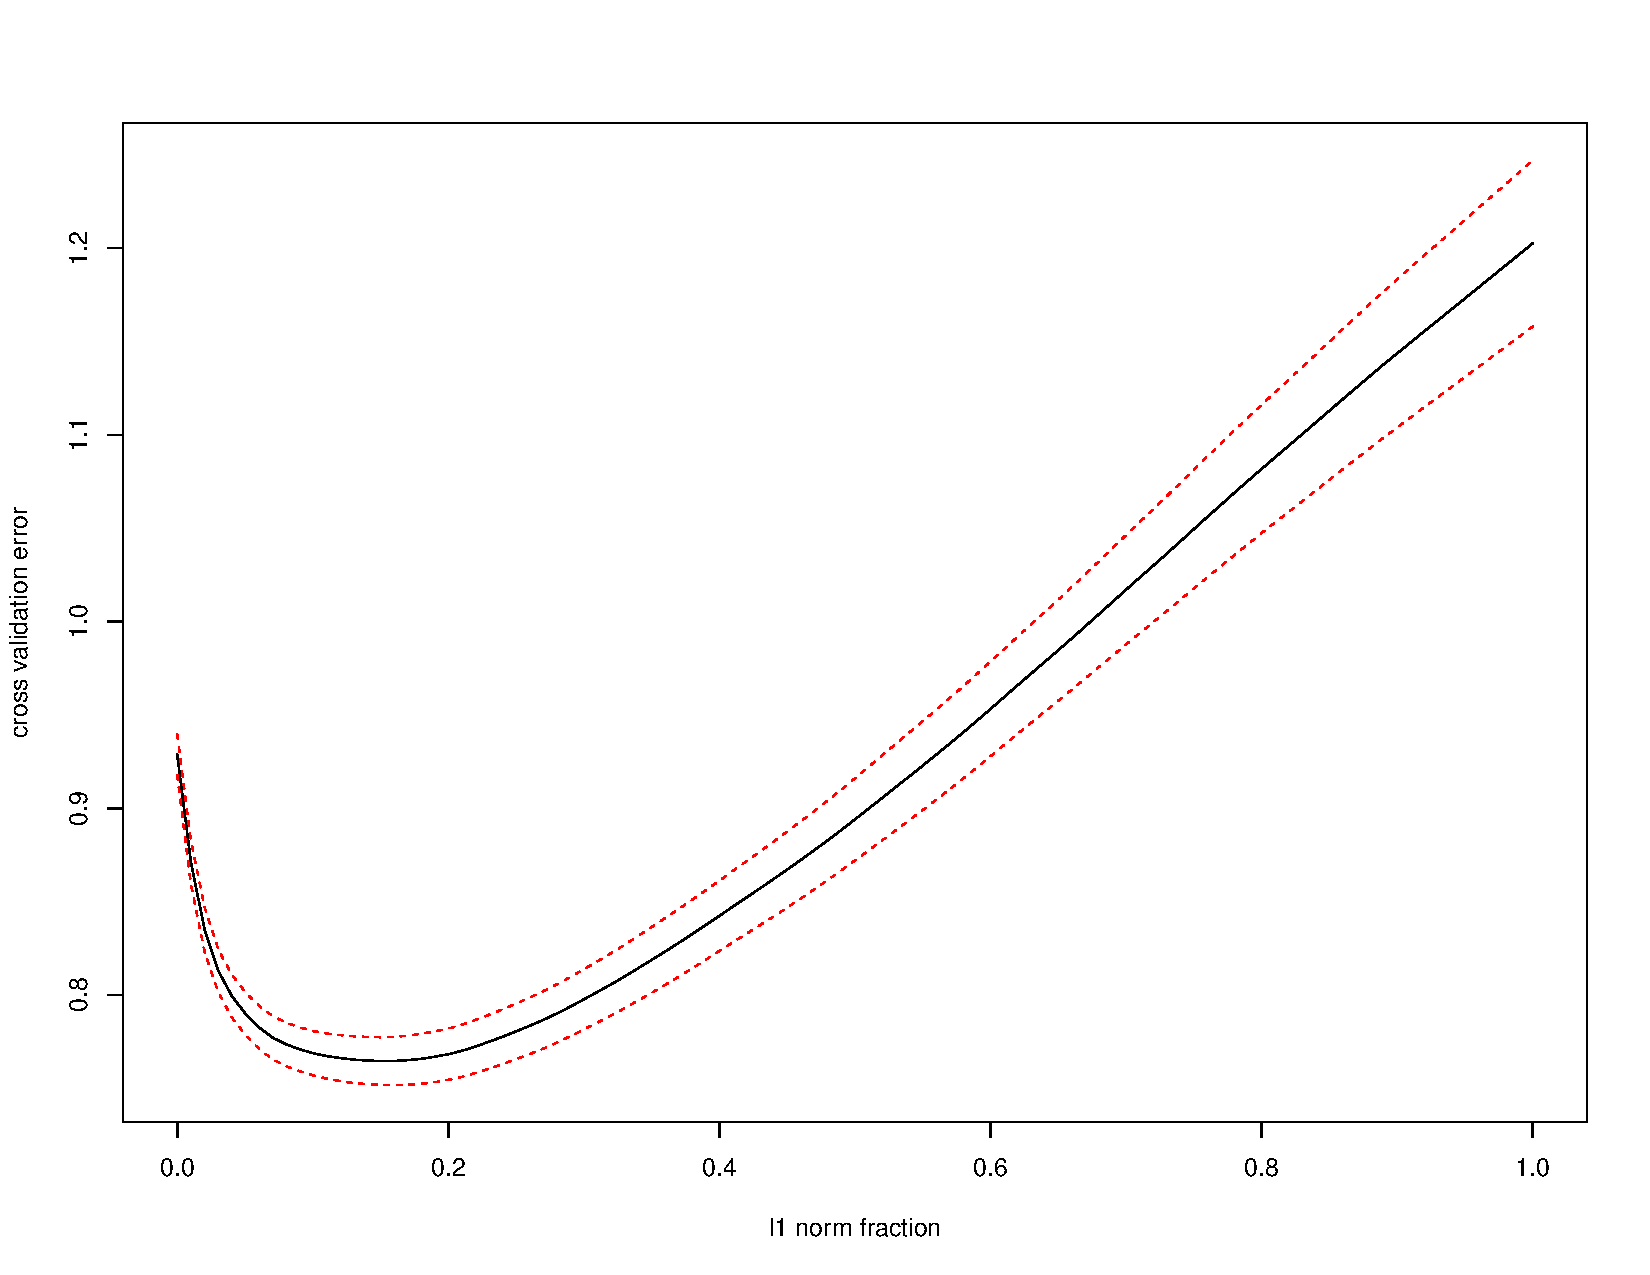
\includegraphics[width=0.8\textwidth]{../lassoResults/CVPosErr.pdf} 
      \caption{Cross-validation error plot for the positive v.s. nonpositive classification. }
   \label{fig:cvplotpos}
\end{figure}
\end{center}

%%%
\subsection{Sparse Regression with LASSO}

LASSO (\cite{tibshirani1996regression}) is a sparse regression method which adds a $l_1$-norm penalty to the linear least squares objective to promote sparsity in the regression coefficients:
\begin{align}
\label{eq:Lasso}
\hat{\beta}(\lambda) = \arg \min_\beta \frac{1}{2}||y-(\beta_0+X\beta)||_2^2 + \lambda ||\beta||_1
\end{align}
In our study, we regress the class label vector $y$ onto the word frequency matrix $X$, yielding the intercept $\hat{\beta_0}$ and the sparse regression vector $\hat{\beta}(\lambda)$. The classifier can be determined to be $f(x) = \textbf{sign}(\hat{\beta_0}+\hat{\beta}^Tx)\in\{-1,+1\}$, where the resulting coefficient regression coefficient $\hat{\beta}$ has the following explanation: for each feature or word $j$, given all other feature or word variables fixed, the increase of the $j$-th word frequency by one leads to an increase in the regression function $\beta_0+\beta^Tx$ by an amount of $\beta_i$ (if $\beta_i$ turns out to be positive, this means the chance of classifying the data point into the $+1$ category is increased).

To look at which words were most relevant to each category we modeled (positive, negative, neutral, and spam), we looked at three sets of 20 words based on, respectively, the highest absolute $\beta$ values, highest positive coefficient values and most negative coefficient values. The top 20 words based on the top 20 highest absolute $\beta$ values tell us in general which words were most relevant to predicting that particular category.  The top 20 words based on the top 20 highest positive $\beta$ values tell us which words typically were common in posts that fell into the category modeled while the top 20 words based on the top 20 largest (in terms of magnitude) negative $\beta$ values tell us which words typically were not in posts that fell into the category modeled but were rather more common in the categories outside of the one we were modeling.

Since the estimated $\beta$ depends on the regularization parameter, we are left with the issue of choosing the ``best'' $\lambda$. A commonly used approach is to do a grid search for $\lambda$: for each value of $\lambda$, do a 10-fold cross validation; then choose the $\lambda$ that yields the smallest cross validation testing sample error. For this method, we used the approach least-angle regression (LARS) by \cite{efron2004least} to do the model selection. Their {\sffamily R} package {\sffamily lars} efficiently fits an entire lasso sequence with the least squares loss function (\cite{Rlars}). Figure~\ref{fig:cvplotpos} shows the cross-validation error plot for the positive v.s. nonpositive classification and the other plots are in Appendix~\ref{asec:cverror}.


%%%
%\note{
%To Angie: include the one of the CV plot here(the positive case); and include the others in the appendix.
%
%To Christine: shorten the following paragraphs...just give some examples for the positive and negative part.
%change 20 to 5, and say the complete lists of words can be found in the appendix
%}



The lists of top 5 most relevant words for positive and negative classification are in Tables~\ref{tb:lassopos}--\ref{tb:lassoneg}.
The complete list of top 20 most relevant words for each classification is in Appendix~\ref{asec:lassowordimages} (Tables~\ref{tb:lassofullpos}--\ref{tb:lassofullspam}).


For the positive responses, the top 5 most relevant words (based on taking the absolute values of the betas) returned by our model are shown in Table~\ref{tb:lassopos}. As can be seen, the top 5 most relevant words for the positive betas and the absolute value of betas were the same. The top 5 relevant words for the two categories have an assortment of fairly neutral or positive words. For example, words such as ``mature,'' ``support,'' and ``keep up the good work'' are very positive in nature and would certainly indicate a positive reaction to 韓寒. The top 5 most relevant words for the negative betas were not as easily classified since the phrases need to be placed in appropriate contexts to be able to tell the sentiment.  We'd expect these words to indicate a dislike of Han han.  An example of how "love" could indicate a dislike of Han Han is the fact that many opponents of Han Han mocked and teased him about his relationship with another author; they'd insinuate that the two authors were lovers.

For the negative responses, the top 5 most relevant words (based on taking the absolute values of the betas) returned by our model are shown in Table~\ref{tb:lassoneg}. As can be seen, the top 5 most relevant words for the positive betas and the absolute value of betas are the same again.  These words clearly hold a negative sentiment.  Words like ``disgusting,'' ``hate,'' and ``liar'' easily suggest that the post exudes a negative sentiment towards the author. The top 5 most relevant words for the negative betas are again a bit harder to classify though looking at the full list of the betas indicates a clearer picture of the fact that negative betas typically correspond to positive words.  The word corresponding to the highest negative coefficient is ``support" which easily indicates a support of Han han. What is interesting to note with these betas is the fact that these betas are all close to zero except for the first phrase.

\begin{table}[!h]
\caption{LASSO word images for the positive v.s. nonpositive classification.}
\begin{center}
\begin{tabular}{|c|c||c|c||c|c|}
\hline
Word & Absolute Coef. & Word & Positive Coef. & Word & Negative Coef.\\ \hline \hline
加油 & 0.820 & 加油 & 0.820 & 样子 & -0.396\\
(keep going) & & (keep going) & & (manner) & \\\hline
韩少 & 0.644 & 韩少 & 0.644 & 恋 & -0.344\\
(Master Han) & & (Master Han) & & (love) & \\\hline
成熟 & 0.546 & 成熟 & 0.546 & 发表 & -0.336\\
(mature) & & (mature) & & (announce) & \\\hline
顶 & 0.533 & 顶 & 0.533 & 道理 & -0.336\\
(support) & & (support) & & (rational) & \\\hline
宽容 & 0.518 & 宽容 & 0.518 & 利益 & -0.335\\
(tolerant) & & (tolerant) & & (benefit) & \\\hline
\end{tabular}
\label{tb:lassopos}
\end{center}
\end{table}



\begin{table}[!h]
\caption{LASSO word images for the negative v.s. nonnegative classification.}
\begin{center}
\begin{tabular}{|c|c||c|c||c|c|}
\hline
Word & Absolute Coef. & Word & Positive Coef. & Word & Negative Coef.\\ \hline \hline
讨厌 & 0.481 & 讨厌 & 0.481 & 支持 & -0.008\\
(hate) & & (hate) & & (support) & \\\hline
无耻 & 0.412 & 无耻 & 0.412 & - & -\\
(shameless) & & (shameless) & & (-) & \\\hline
恶心 & 0.395 & 恶心 & 0.395 & - & -\\
(disgusting) & & (disgusting) & &  & \\\hline
骗子 & 0.380 & 骗子 & 0.380 & - & -\\
(liar) & & (liar) & &  & \\\hline
扁 & 0.353 & 扁 & 0.353 & - & -\\
(beat up) & & (beat up) & &  & \\\hline
\end{tabular}
\label{tb:lassoneg}
\end{center}
\end{table}

%
%\begin{table}
%\caption{LASSO word images for the neutral  v.s. nonneutral classification.}
%\begin{center}
%\begin{tabular}{|c|c||c|c||c|c|}
%\hline
%Word & Absolute Coef. & Word & Positive Coef. & Word & Negative Coef.\\ \hline
%上调 & 0.586 & 上调 & 0.586 & 加油 & -0.491\\
%(increase) & & (increase) & & (keep going) & \\\hline
%道理 & 0.566 & 道理 & 0.566 & 韩少 & -0.358\\
%(rational) & & (rational) & & (Master Han) & \\\hline
%账号 & 0.534 & 账号 & 0.534 & 苦肉计 & -0.327\\
%(account) & & (account) & & (the ruse of  & \\
%& &  & &  self-injury to win & \\
%& &  & &  somebody's & \\
%& &  & &   confidence) & \\\hline
%加油 & 0.491 & 铁证 & 0.459 & 支持 & -0.290\\
%(keep going) & & (clear evidence) & & (support) & \\\hline
%铁证 & 0.459 & 称 & 0.453 & 善良 & -0.268\\
%(clear evidence) & & (refer) & & (kind) & \\\hline
%\end{tabular}
%\label{tb:lassoneu}
%\end{center}
%\end{table}
%
%
%\begin{table}
%\caption{LASSO word images for the spam  v.s. nonspam classification.}
%\begin{center}
%\begin{tabular}{|c|c||c|c||c|c|}
%\hline
%Word & Absolute Coef. & Word & Positive Coef. & Word & Negative Coef.\\ \hline
%查看 & 3.777 & 查看 & 3.777 & 韩少 & -1.033\\
%(examine) & & (examine) & & (Master Hanhan) & \\\hline
%抽 & 1.998 & 抽 & 1.998 & 韩寒 & -0.716\\
%(win) & & (win) & & (Master Hanhan) & \\\hline
%每天 & 1.251 & 每天 & 1.251 & 别 & -0.232\\
%(everyday) & & (everyday) & & (don't) & \\\hline
%往往 & 1.208 & 往往 & 1.208 & 支持 & -0.217\\
%(often) & & (often) & & (support) & \\\hline
%外 & 1.043 & 外 & 1.043 & 这种 & -0.202\\
%(outside) & & (outside) & & (this kind) & \\\hline
%\end{tabular}
%\label{tb:lassospam}
%\end{center}
%\end{table}

%%%%%%%%%%%%%%%%%%%%%%%%%%%%%%%%%%%%%%%%
\subsection{$l_1$-Norm Support Vector Machine}

The support vector machine (SVM) is another commonly used machine learning method to classify data points into two categories. Consider again the linear decision function $f(x) = \beta_0 + \beta^T x$ and the sign classifier $\text{class}(x) = \textbf{sign} (f(x))$. The SVM minimizes the training misclassification rate and the margin of the decision boundary. Following the notations in \cite{hastie2004entire}:
\begin{align}
\label{eq:l2svm}
\min_{\beta_0,\beta} \sum_{i=1}^n(1-y_i(\beta_0+\beta^Tx_i))_+ + \frac{\lambda}{2} ||\beta||_2^2,
\end{align}
where $z_+ = \max(0,z)$ (the function $h(z) = (1-z)_+$ is also known as the hinge loss function). Similarly, the sparse version of SVM simply replaces the $l_2$-norm by $l_1$-norm (see, e.g. \cite{zhu20041}):
\begin{align*}
\label{eq:l1svm}
\min_{\beta_0,\beta} \left\{ \sum_{i=1}^n(1-y_i(\beta_0+\beta^Tx_i))_+ + \lambda ||\beta||_1\right\}. 
\end{align*}
We repeat the same data analysis for the text data using $l_1$-norm SVM as we did for the LASSO classification. To fit the sparse SVM, we use the matlab package {\tt lpsvm} by \cite{fung2004feature}. Again, 10-fold cross validations are performed in order to select the regularization parameter $\lambda$. Again the model seems to produce plausible results. Also, the top coefficients obtained by $l_1$-norm SVM seems to be consistent with those obtained by fitting a LASSO.  

%We repeat the same data analysis for the text data using $l_1$-norm SVM as we did for the LASSO classification. The results are summarized in Table XX. To fit the sparse SVM, we use the matlab package {\tt lpsvm} by \cite{fung2004feature}. Again, 10-fold cross validations are performed in order to select the regularization parameter $\lambda$. Again the model seems to produce plausible results. Also, the top coefficients obtained by $l_1$-norm SVM seem to be consistent with those obtained by fitting a LASSO.  
%
%\note{
%To Angie:
%include the four tables here(each of top five words)... and rest in the appendix
%}

The lists of top 5 most relevant words for positive and negative classification are in Tables~\ref{tb:svmpos}--\ref{tb:svmneg}.
The complete list of top 20 most relevant words for each classification is in Appendix~\ref{asec:svmwordimages} (Tables~\ref{tb:svmfullpos}--\ref{tb:svmfullspam}).

\begin{table}[!h]
\caption{$l_1$-norm SVM word images for the positive v.s. nonpositive classification.}
\begin{center}
\begin{tabular}{|c|c||c|c||c|c|}
\hline
Word & Absolute Coef. & Word & Positive Coef. & Word & Negative Coef.\\ \hline \hline
加油 & 2.340 & 加油 & 2.340 & 铁证 & 2.305\\
(keep going) & & (keep going) & & (clear evidence) & \\\hline
铁证 & 2.305 & 家人 & 2.269 & 接受 & 2.061\\
(clear evidence) & & (family) & & (accept) & \\\hline
家人 & 2.269 & 韩少 & 1.969 & 媒体 & 1.907\\
(family) & & (Master Han) & & (media) & \\\hline
接受 & 2.061 & 成熟 & 1.806 & 默默 & 1.883\\
(accept) & & (mature) & & (quietly) & \\\hline
韩少 & 1.969 & 顶 & 1.803 & 四娘 & 1.762\\
(Master Han) & & (support) & & (GUO Jingming) & \\\hline
\end{tabular}
\label{tb:svmpos}
\end{center}
\end{table}



\begin{table}
\caption{$l_1$-norm SVM word images for the negative v.s. nonnegative classification.}
\begin{center}
\begin{tabular}{|c|c||c|c||c|c|}
\hline
Word & Absolute Coef. & Word & Positive Coef. & Word & Negative Coef.\\ \hline  \hline
扁 & 1.777 & 扁 & 1.777 & 脑子 & 1.447\\
(beat up) & & (beat up) & & (mind) & \\\hline
苦肉计 & 1.708 & 苦肉计 & 1.708 & 彻底 & 1.290\\
(the ruse of  & & (the ruse of  &  &  (completely) &  \\
self-injury to win & &  self-injury to win &  & &  \\
somebody's & & somebody's  &  & &  \\
 confidence) & &  confidence)  &  & &  \\\hline
恶心 & 1.527 & 恶心 & 1.527 & 送给 & 1.221\\
(disgusting) & & (disgusting) & & (give) & \\\hline
脑子 & 1.447 & 骗子 & 1.301 & 感觉 & 1.109\\
(asdf) & & (liar) & & (feel) & \\\hline
骗子 & 1.301 & 公开 & 1.220 & 热点 & 1.101\\
(liar) & & (open) & & (hot interest) & \\\hline
\end{tabular}
\label{tb:svmneg}
\end{center}
\end{table}


%\begin{table}
%\caption{$l_1$-norm support vector machine results: neutral category}
%\begin{center}
%\begin{tabular}{|c|c||c|c||c|c|}
%\hline
%Word & Absolute Coef. & Word & Positive Coef. & Word & Negative Coef.\\ \hline\hline
%加油 & 2.233 & 铁证 & 2.054 & 加油 & 2.233\\
%(keep going) & & (clear evidence) & & (keep going) & \\\hline
%铁证 & 2.054 & 片 & 1.896 & 成熟 & 1.756\\
%(clear evidence) & & (piece) & & (mature) & \\\hline
%片 & 1.896 & 至今 & 1.884 & 同意 & 1.725\\
%(piece) & & (so far) & & (agree) & \\\hline
%至今 & 1.884 & 战 & 1.845 & 水 & 1.661\\
%(so far) & & (fight) & & (water) & \\\hline
%战 & 1.845 & 意思 & 1.824 & 昨天 & 1.611\\
%(fight) & & (meaning) & & (yesterday) & \\\hline
%\end{tabular}
%\end{center}
%\end{table}
%
%
%
%
%\begin{table}
%\caption{$l_1$-norm support vector machine results: spam category}
%\begin{center}
%\begin{tabular}{|c|c||c|c||c|c|}
%\hline
%Word & Absolute Coef. & Word & Positive Coef. & Word & Negative Coef.\\ \hline\hline
%票子 & 1.000 & 票子 & 1.000 & 书 & 0.000\\
%(ticket) & & (ticket) & & (book) & \\\hline
%书 & 0.000 & 每天 & 0.000 & 围观 & 0.000\\
%(book) & & (everyday) & & (surround to watch) & \\\hline
%围观 & 0.000 & 抽 & 0.000 & 写 & 0.000\\
%(surround to watch) & & (win) & & (write) & \\\hline
%写 & 0.000 & 性 & 0.000 & 骂 & 0.000\\
%(write) & & (sex) & & (curse) & \\\hline
%每天 & 0.000 & 网 & 0.000 & 粉丝 & 0.000\\
%(everyday) & & (Internet) & & (fans) & \\\hline
%\end{tabular}
%\end{center}
%\end{table}

\clearpage
%%%%%%%
\section{Test Set Misclassification Rates}

To compare the classification performance, we use the best fitted models discussed above to classify the test set of 500 posts. Recall that the best models are selected to minimize the 10-fold cross validation error. Table~\ref{tb:testcounts} shows the frequency count of each category in the 500 posts and Table~\ref{tb:testmis} summarizes the test results. 

\begin{table}[!h]
\caption{Counts of posts in each of the four categories among the 500 test posts.}
\begin{center}
\begin{tabular}{|c|c|c|c|}
\hline
Positive & Negative & Neutral & Spam \\ \hline
 172      & 36   &   287   &  5 \\ \hline
\end{tabular}
\end{center}
\label{tb:testcounts}
\end{table}%


\begin{table}[!h]
\caption{Misclassification rates of the three methods for each of the four categories.}
\begin{center}
\begin{tabular}{|c|c|c|c|c|}
\hline
              &  			Positive & Negative & Neutral & Spam  \\ \hline
Sentiment score assignment & 	78.6\%		&	97.2\%	&  78.8\%	& -  \\ \hline
LASSO               & 	22.6\%   &   7\%   &   33.6\%    &    1\% \\ \hline
$l_1$-norm SVM       &       22.6\%  &    8\%    &  33.4\%   &     1\% \\ \hline
\end{tabular}
\end{center}
\label{tb:testmis}
\end{table}%



It can be seen that the two standard machine learning methods produce very similar results. Also notice the low misclassification rates in the negative and spam categories, which might be due to the fact that we do not frequently see posts that belong to those two categories in our test set.



It is also surprising to see how the sentiment score assignment method fails miserably in classifying the posts. As discussed in Section~\ref{subsec:senscore}, this na\"\i ve approach is dictionary-based and only considers the individual words. Clearly an entity is not merely the sum of its parts. It is crucial to take context into account in sentiment analysis. For instance, a post containing many positive words may be praising Fang Zhouzi and hence against Han Han.  Moverover, zero score has two scenarios: the post contains the same number of positive  and negative words; there is no sentimental words presented. Even though these two cases can be distinguished, there is still little information to make reasonable inference. Since the dictionary itself is limited, the scores may not represent the whole picture.

%\note{Perhaps Angie wants to say more here.....}

%\clearpage
%%%%%%%%%%%%%%%%%%
\section{Conclusion}

In this project, we developed a framework for studying public opinions using Sina Weibo as a corpus for a given topic. Posts are collected from Weibo and then processed taking the characteristics of both the Chinese language and Weibo posts into consideration. Also the processing is topic-dependent since there are certain proper nouns related to a given topic.
Word usage relation has been examined. Due to the sparsity of the word frequency matrix, both sparse principle component analysis  (SPCA) and sparse graphical models are employed in our feature analysis. 
Two standard machine learning methods, namely sparse regression with LASSO and $l_1$-norm SVM, have been applied to the training set of 3,000 posts and then the best fitted models are tested on a test set of 500 posts. These two methods have similar performance on our data set. Due to limitation in time we have not extented our study to a larger corpus. However, the sparse machine learning tools we have used in this project produce human-interpretable results and reasonable misclassification rates.

Many future efforts remain to be done. One possible direction is to enlarge the scale of our study, in both time (i.e. extend the time period we do the sampling) and number of posts. In terms of sampling techniques, we would like to study random samples by sampling from large network as discussed in Section~\ref{subsec:datacol} after spams, OOV, and reposting can be handled properly. In terms of methodology, we would like to compare our LASSO and $l_1$-norm SVM methods with the popular maximum entropy approach \cite{lee2011chinese, nigam1999using}. Also, as discussed in Section~\ref{subsec:datacol}, one topic of interest is to track repostings using graphical models. Identification of OOV needs more statistical work as well.  Clearly sentiment classifier is topic-dependent and there is no reason why we should restrict our analysis on just a few famous public figures. In the future, we can collect data on more and broader topics, preferably in other domains, to test our framework.
\clearpage

\newpage
\newpage
%%%%%%%%%%%%%
% bibliography
\bibliographystyle{apalike}
\bibliography{215B_FinalProjRef}


\newpage
%%%%%%%%%%%%%%%%%%
\appendix
\section{Sparse graphical model plots}

\begin{center}
\begin{figure}[tb]
   \centering
   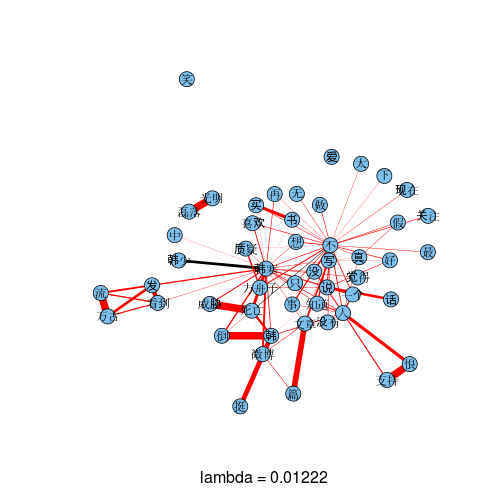
\includegraphics[width=0.7\textwidth]{../gLassoResults/glasso2.png} 
      \caption{ }
   \label{fig:glasso2}
\end{figure}
\end{center}

\begin{center}
\begin{figure}[tb]
   \centering
   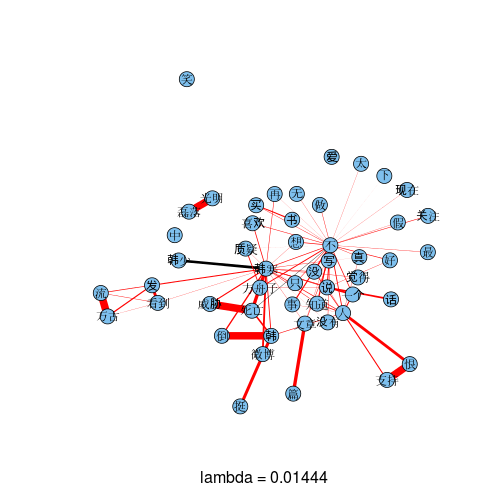
\includegraphics[width=0.7\textwidth]{../gLassoResults/glasso3.png} 
      \caption{ }
   \label{fig:glasso3}
\end{figure}
\end{center}

\begin{center}
\begin{figure}[tb]
   \centering
   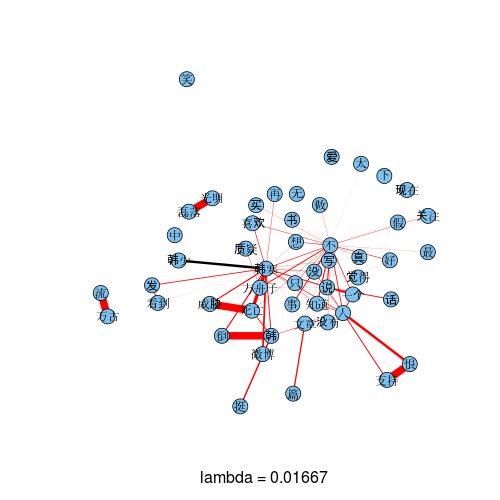
\includegraphics[width=0.7\textwidth]{../gLassoResults/glasso4.png} 
      \caption{ }
   \label{fig:glasso4}
\end{figure}
\end{center}

\begin{center}
\begin{figure}[tb]
   \centering
   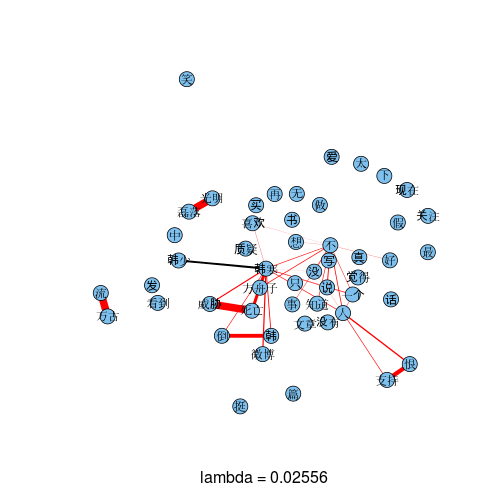
\includegraphics[width=0.7\textwidth]{../gLassoResults/glasso5.png} 
      \caption{ }
   \label{fig:glasso5}
\end{figure}
\end{center}

\begin{center}
\begin{figure}[tb]
   \centering
   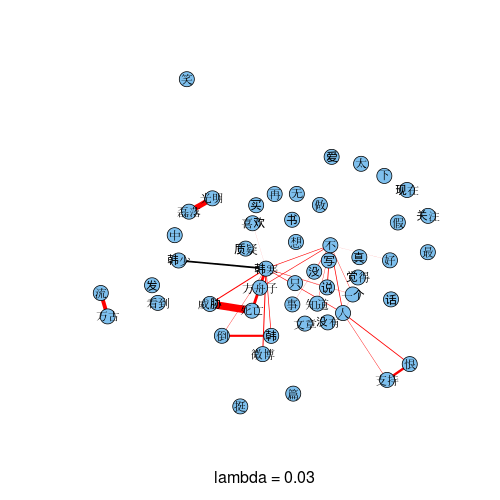
\includegraphics[width=0.7\textwidth]{../gLassoResults/glasso6.png} 
      \caption{ }
   \label{fig:glasso6}
\end{figure}
\end{center}


%%%%%
\section{LASSO Results}

%%%
\subsection{Cross-Validation Error Plot}\label{asec:cverror}

\begin{center}
\begin{figure}[!h]
   \centering
   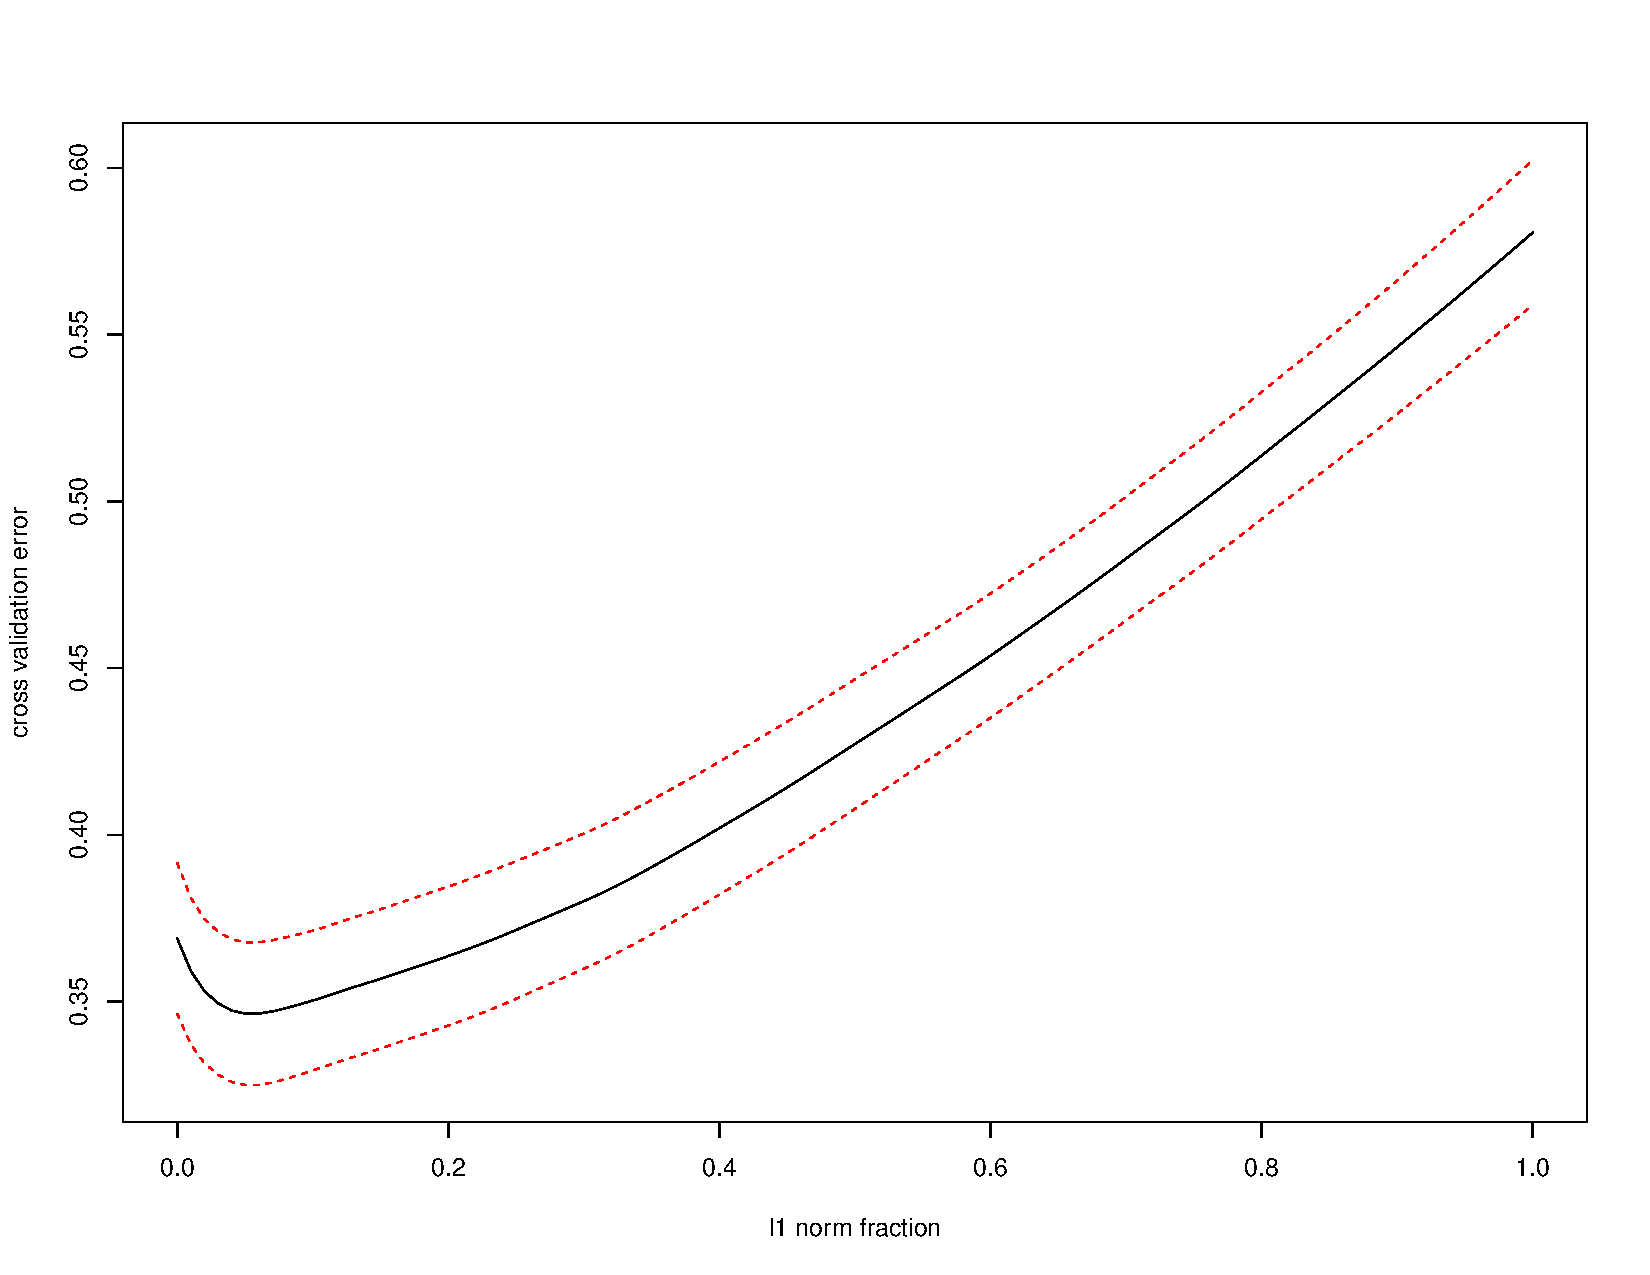
\includegraphics[width=0.7\textwidth]{../lassoResults/CVNegErr.pdf} 
      \caption{Cross-validation error plot for the negative v.s. nonnegative classification. }
   \label{fig:cvplotneg}
\end{figure}
\end{center}

\begin{center}
\begin{figure}[!h]
   \centering
   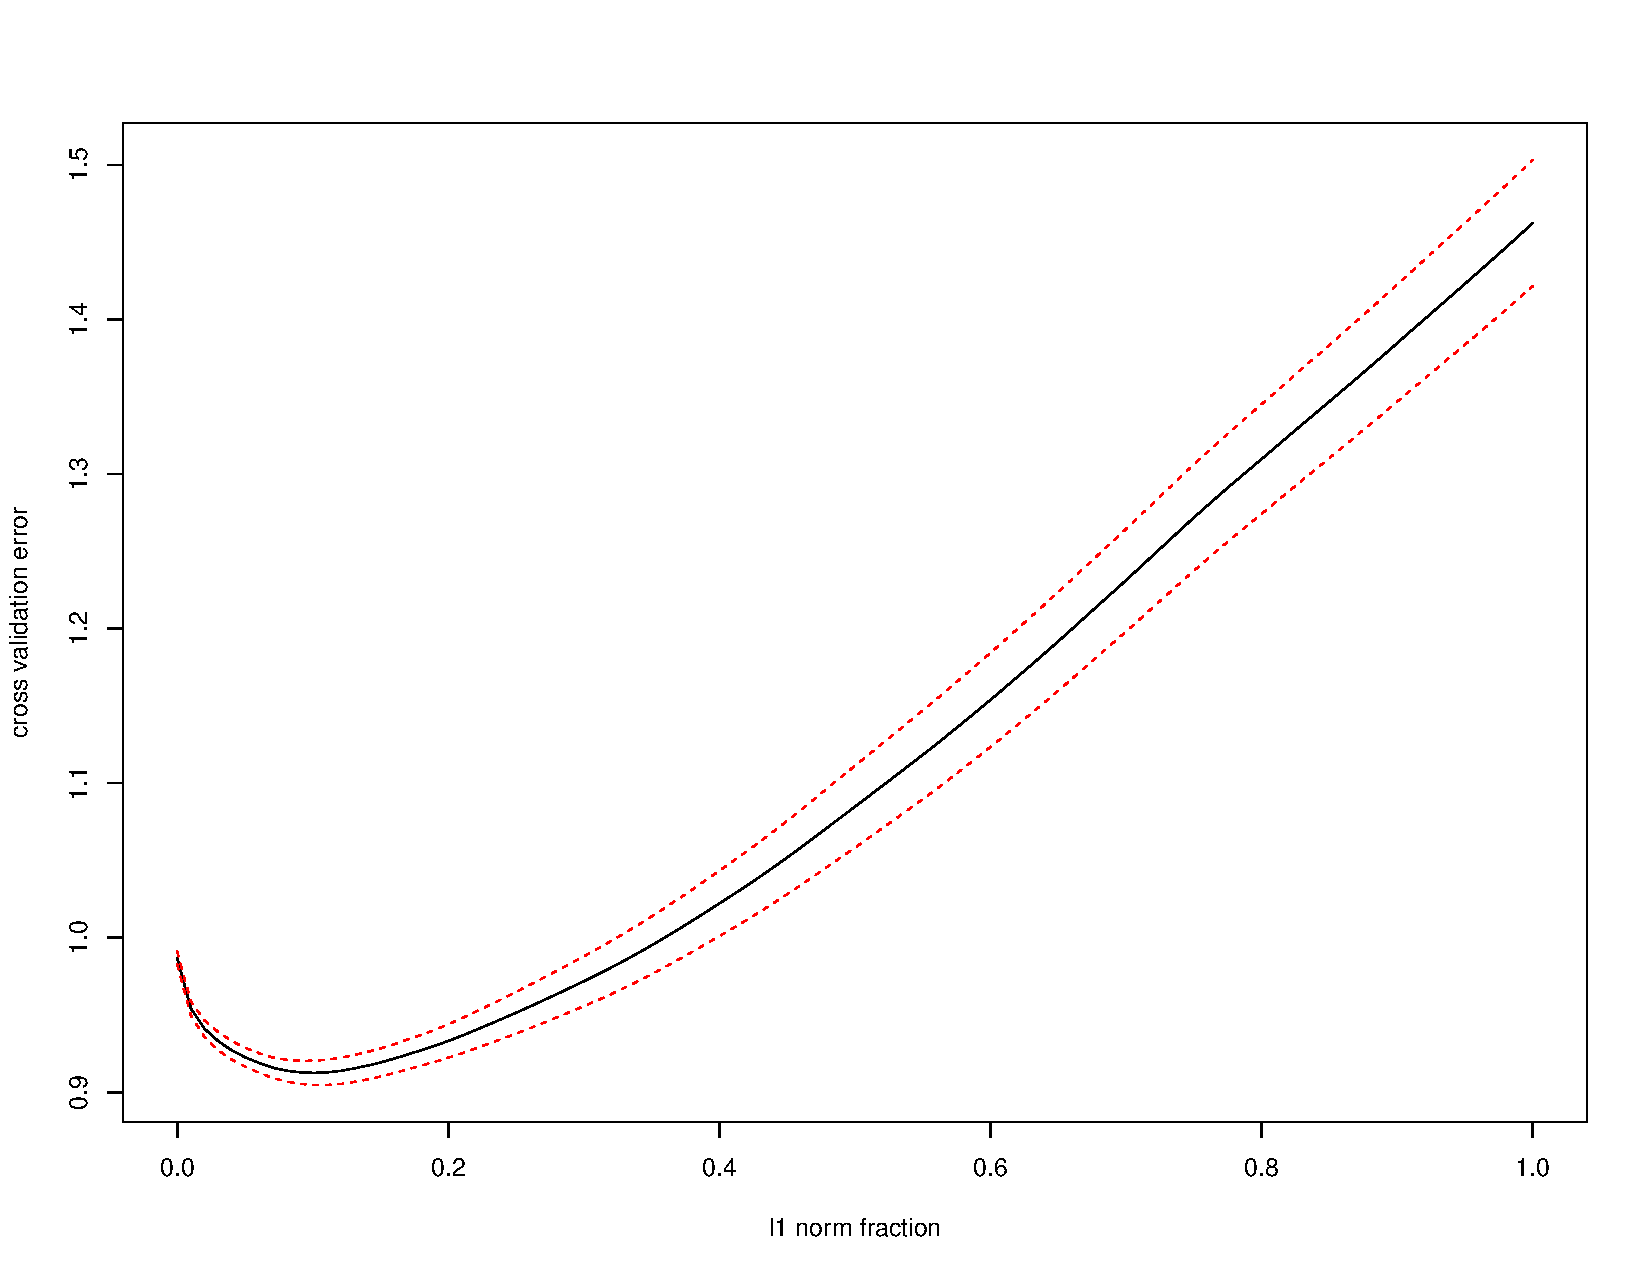
\includegraphics[width=0.7\textwidth]{../lassoResults/CVNeuErr.pdf} 
      \caption{Cross-validation error plot for the neutral v.s. nonneutral classification. }
   \label{fig:cvplotneu}
\end{figure}
\end{center}

\begin{center}
\begin{figure}[!h]
   \centering
   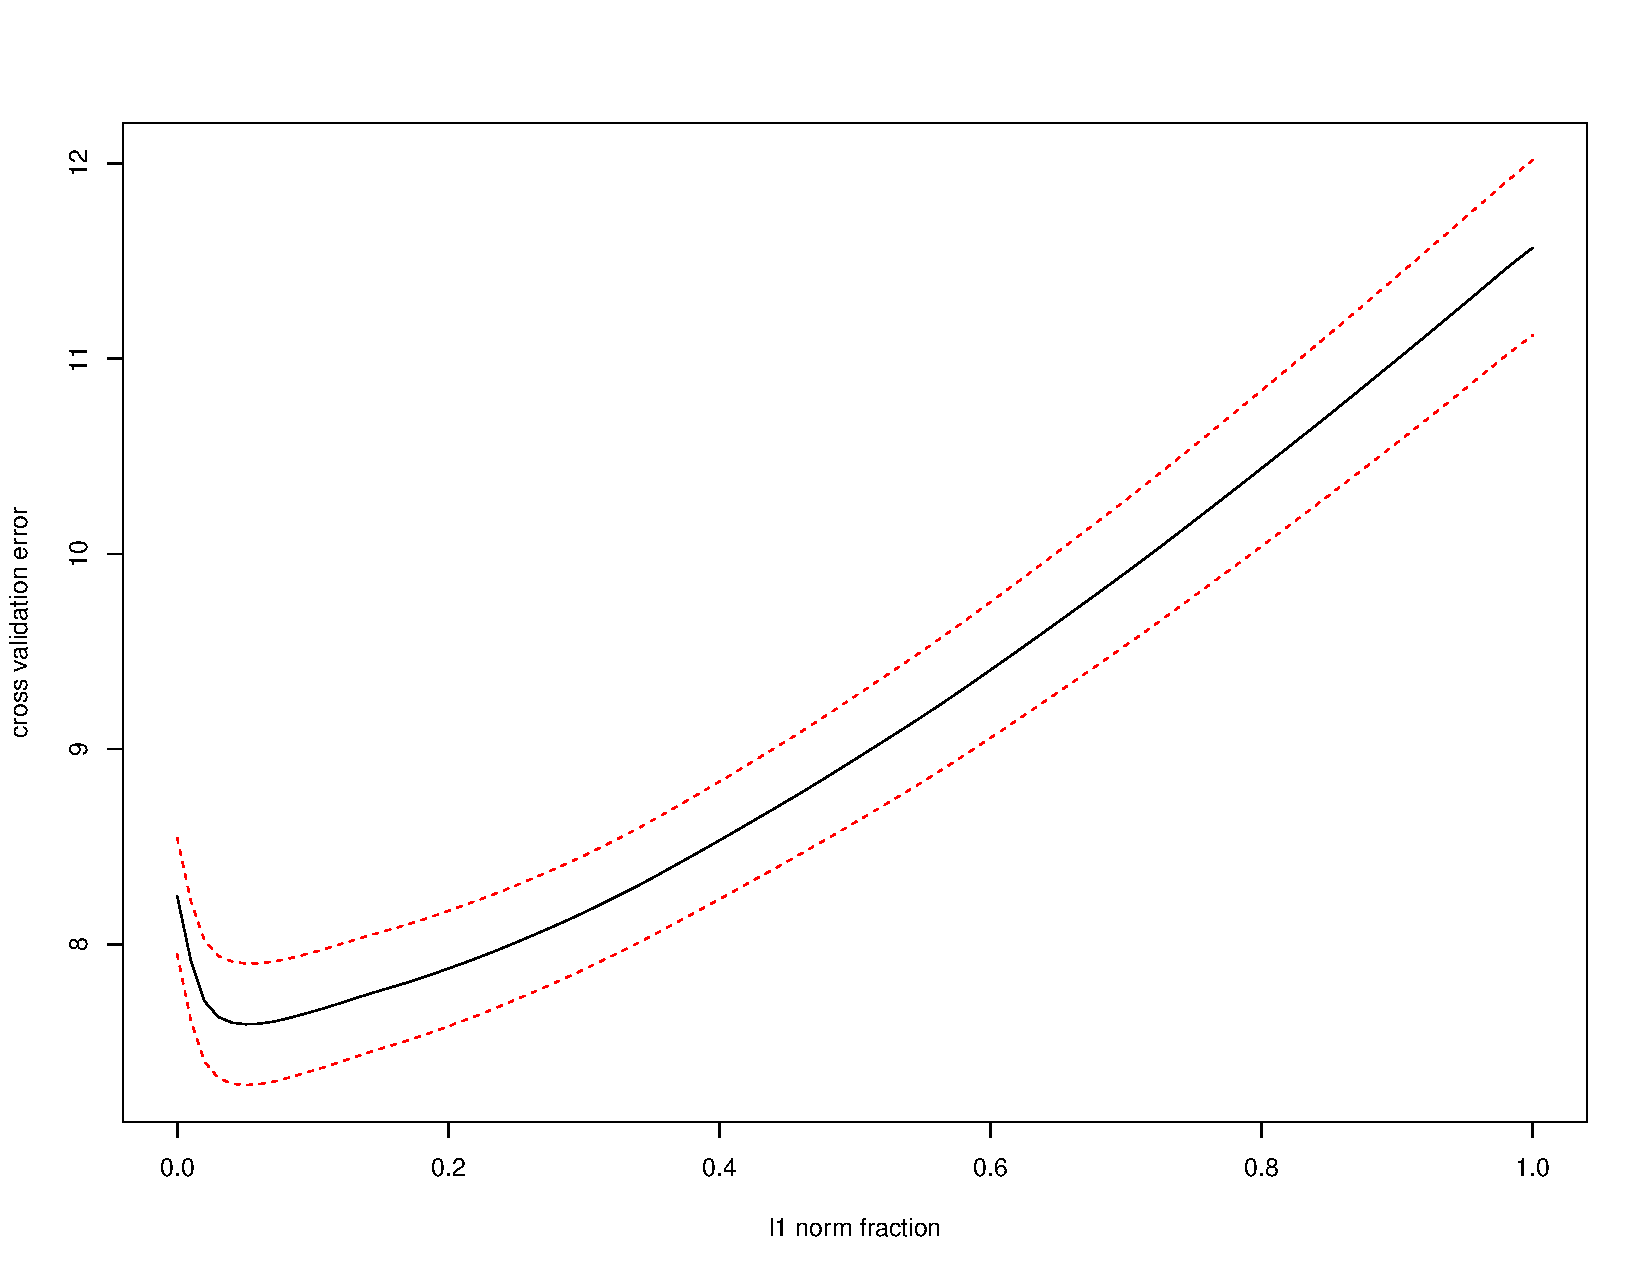
\includegraphics[width=0.7\textwidth]{../lassoResults/CVSpamErr.pdf} 
      \caption{Cross-validation error plot for the spam v.s. nonspam classification. }
   \label{fig:cvplotspam}
\end{figure}
\end{center}

\clearpage
\newpage
%%
\subsection{LASSO Word Images}\label{asec:lassowordimages}

\begin{table}[!h]
\caption{LASSO word images for the positive v.s. nonpositive classification.}
\begin{center}
\begin{tabular}{|c|c||c|c||c|c|}
\hline
Word & Absolute Coef. & Word & Positive Coef. & Word & Negative Coef.\\ \hline \hline
加油 & 0.820 & 加油 & 0.820 & 样子 & -0.396\\
(keep going) & & (keep going) & & (manner) & \\\hline
韩少 & 0.644 & 韩少 & 0.644 & 恋 & -0.344\\
(Master Han) & & (Master Han) & & (love) & \\\hline
成熟 & 0.546 & 成熟 & 0.546 & 发表 & -0.336\\
(mature) & & (mature) & & (announce) & \\\hline
顶 & 0.533 & 顶 & 0.533 & 道理 & -0.336\\
(support) & & (support) & & (rational) & \\\hline
宽容 & 0.518 & 宽容 & 0.518 & 利益 & -0.335\\
(tolerant) & & (tolerant) & & (benefit) & \\\hline
支持 & 0.477 & 支持 & 0.477 & 称 & -0.323\\ \hline
家人 & 0.467 & 家人 & 0.467 & 遭受 & -0.323\\ \hline
样子 & 0.396 & 尤其 & 0.395 & 媒体 & -0.319\\ \hline
尤其 & 0.395 & 欣赏 & 0.383 & 翻 & -0.314\\ \hline
欣赏 & 0.383 & 感动 & 0.381 & 铁证 & -0.289\\ \hline
感动 & 0.381 & 影响力 & 0.370 & 骗子 & -0.248\\ \hline
影响力 & 0.370 & 新书 & 0.327 & 上调 & -0.248\\ \hline
恋 & 0.344 & 铁 & 0.316 & 投票 & -0.234\\ \hline
发表 & 0.336 & 不错 & 0.309 & 女 & -0.230\\ \hline
道理 & 0.336 & 终于 & 0.274 & 四娘 & -0.226\\ \hline
利益 & 0.335 & 每个 & 0.274 & 关系 & -0.215\\ \hline
新书 & 0.327 & 咬 & 0.261 & 广告 & -0.210\\ \hline
称 & 0.323 & 文字 & 0.260 & 接受 & -0.208\\ \hline
遭受 & 0.323 & 蛋 & 0.244 & 网 & -0.204\\ \hline
媒体 & 0.319 & 纠缠 & 0.244 & 底 & -0.196\\ \hline
\end{tabular}
\label{tb:lassofullpos}
\end{center}
\end{table}



\begin{table}[!h]
\caption{LASSO word images for the negative v.s. nonnegative classification.}
\begin{center}
\begin{tabular}{|c|c||c|c||c|c|}
\hline
Word & Absolute Coef. & Word & Positive Coef. & Word & Negative Coef.\\ \hline \hline
讨厌 & 0.481 & 讨厌 & 0.481 & 支持 & -0.008\\
(hate) & & (hate) & & (support) & \\\hline
无耻 & 0.412 & 无耻 & 0.412 & 不 & 0.000\\
(shameless) & & (shameless) & & (no) & \\\hline
恶心 & 0.395 & 恶心 & 0.395 & 人 & 0.000\\
(disgusting) & & (disgusting) & & (people/person) & \\\hline
骗子 & 0.380 & 骗子 & 0.380 & 说 & 0.000\\
(liar) & & (liar) & & (say) & \\\hline
扁 & 0.353 & 扁 & 0.353 & 方舟子 & 0.000\\
(beat up) & & (beat up) & & (FangZhouZi) & \\\hline
装 & 0.321 & 装 & 0.321 & 韩少 & 0.000\\ \hline
选项 & 0.292 & 选项 & 0.292 & 真 & 0.000\\ \hline
苦肉计 & 0.290 & 苦肉计 & 0.290 & 好 & 0.000\\ \hline
利益 & 0.283 & 利益 & 0.283 & 没 & 0.000\\ \hline
全 & 0.261 & 全 & 0.261 & 一个 & 0.000\\ \hline
国家 & 0.247 & 国家 & 0.247 & 微博 & 0.000\\ \hline
智商 & 0.216 & 智商 & 0.216 & 写 & 0.000\\ \hline
告 & 0.198 & 告 & 0.198 & 喜欢 & 0.000\\ \hline
虚伪 & 0.192 & 虚伪 & 0.192 & 想 & 0.000\\ \hline
演 & 0.191 & 演 & 0.191 & 威胁 & 0.000\\ \hline
语 & 0.186 & 语 & 0.186 & 只 & 0.000\\ \hline
烦 & 0.178 & 烦 & 0.178 & 太 & 0.000\\ \hline
掉 & 0.142 & 掉 & 0.142 & 事 & 0.000\\ \hline
下去 & 0.141 & 下去 & 0.141 & 没有 & 0.000\\ \hline
公开 & 0.141 & 公开 & 0.141 & 看到 & 0.000\\ \hline
\end{tabular}
\label{tb:lassofullneg}
\end{center}
\end{table}


\begin{table}[!h]
\caption{LASSO word images for the neutral v.s. nonneutral classification.}
\begin{center}
\begin{tabular}{|c|c||c|c||c|c|}
\hline
Word & Absolute Coef. & Word & Positive Coef. & Word & Negative Coef.\\ \hline
上调 & 0.586 & 上调 & 0.586 & 加油 & -0.491\\
(increase) & & (increase) & & (keep going) & \\\hline
道理 & 0.566 & 道理 & 0.566 & 韩少 & -0.358\\
(rational) & & (rational) & & (Master Han) & \\\hline
账号 & 0.534 & 账号 & 0.534 & 苦肉计 & -0.327\\
(account) & & (account) & & (the ruse of  & \\
& &  & &  self-injury to win & \\
& &  & &  somebody's & \\
& &  & &   confidence) & \\\hline
加油 & 0.491 & 铁证 & 0.459 & 支持 & -0.290\\
(keep going) & & (clear evidence) & & (support) & \\\hline
铁证 & 0.459 & 称 & 0.453 & 善良 & -0.268\\
(clear evidence) & & (refer) & & (kind) & \\\hline
称 & 0.453 & 想起 & 0.353 & 成熟 & -0.263\\ \hline
韩少 & 0.358 & 杀 & 0.331 & 终于 & -0.239\\ \hline
想起 & 0.353 & 最终 & 0.329 & 家人 & -0.233\\ \hline
杀 & 0.331 & 意思 & 0.323 & 同意 & -0.228\\ \hline
最终 & 0.329 & 遭遇 & 0.319 & 越来越 & -0.220\\ \hline
苦肉计 & 0.327 & 金 & 0.308 & 欢乐 & -0.217\\ \hline
意思 & 0.323 & 片 & 0.287 & 崇拜 & -0.213\\ \hline
遭遇 & 0.319 & 应 & 0.278 & 讨厌 & -0.202\\ \hline
金 & 0.308 & 变成 & 0.265 & 顶 & -0.197\\ \hline
支持 & 0.290 & 有点 & 0.262 & 代笔 & -0.194\\ \hline
片 & 0.287 & 之间 & 0.254 & 跳 & -0.191\\ \hline
应 & 0.278 & 右边 & 0.250 & 真善美 & -0.186\\ \hline
善良 & 0.268 & 民主 & 0.238 & 真正 & -0.185\\ \hline
变成 & 0.265 & 郭敬明 & 0.237 & 欣赏 & -0.181\\ \hline
成熟 & 0.263 & 久 & 0.226 & 无耻 & -0.180\\ \hline
\end{tabular}
\label{tb:lassofullneu}
\end{center}
\end{table}


\begin{table}[!h]
\caption{LASSO word images for the spam v.s. nonspam classification.}
\begin{center}
\begin{tabular}{|c|c||c|c||c|c|}
\hline
Word & Absolute Coef. & Word & Positive Coef. & Word & Negative Coef.\\ \hline
查看 & 3.777 & 查看 & 3.777 & 韩少 & -1.033\\
(examine) & & (examine) & & (Master Hanhan) & \\\hline
抽 & 1.998 & 抽 & 1.998 & 韩寒 & -0.716\\
(win) & & (win) & & (Master Hanhan) & \\\hline
每天 & 1.251 & 每天 & 1.251 & 别 & -0.232\\
(everyday) & & (everyday) & & (don't) & \\\hline
往往 & 1.208 & 往往 & 1.208 & 支持 & -0.217\\
(often) & & (often) & & (support) & \\\hline
外 & 1.043 & 外 & 1.043 & 这种 & -0.202\\
(outside) & & (outside) & & (this kind) & \\\hline
韩少 & 1.033 & 征集 & 0.948 & 感 & -0.196\\ \hline
征集 & 0.948 & 容 & 0.849 & 韓 & -0.191\\ \hline
容 & 0.849 & 风 & 0.649 & 没有 & -0.179\\ \hline
韩寒 & 0.716 & 票子 & 0.570 & 上调 & -0.174\\ \hline
风 & 0.649 & 考 & 0.540 & 方舟子 & -0.160\\ \hline
票子 & 0.570 & 主 & 0.438 & 光明 & -0.141\\ \hline
考 & 0.540 & 性 & 0.430 & 一定 & -0.137\\ \hline
主 & 0.438 & 总是 & 0.416 & 照妖镜 & -0.132\\ \hline
性 & 0.430 & 儿 & 0.416 & 写 & -0.132\\ \hline
总是 & 0.416 & 结论 & 0.405 & 觉得 & -0.119\\ \hline
儿 & 0.416 & 后面 & 0.397 & 甚 & -0.110\\ \hline
结论 & 0.405 & 法律 & 0.388 & 韩 & -0.092\\ \hline
后面 & 0.397 & 机会 & 0.376 & 真相 & -0.084\\ \hline
法律 & 0.388 & 公知 & 0.357 & 挺 & -0.072\\ \hline
机会 & 0.376 & 中 & 0.357 & 不 & -0.068\\ \hline
\end{tabular}
\label{tb:lassofullspam}
\end{center}
\end{table}


%%%%%%%%%
%%%%%%%%%
\clearpage
\newpage
\section{$l_1$-Norm Support Vector Machine Results}


%%
\subsection{$l_1$-Norm SVM Word Images}\label{asec:svmwordimages}



\begin{table}[!h]
\caption{$l_1$-norm SVM word images for the positive v.s. nonpositive classification.}
\centering
\begin{tabular}{|c|c||c|c||c|c|}
\hline
Word & Absolute Coef. & Word & Positive Coef. & Word & Negative Coef.\\ \hline \hline
加油 & 2.340 & 加油 & 2.340 & 铁证 & 2.305\\
(keep going) & & (keep going) & & (clear evidence) & \\\hline
铁证 & 2.305 & 家人 & 2.269 & 接受 & 2.061\\
(clear evidence) & & (family) & & (accept) & \\\hline
家人 & 2.269 & 韩少 & 1.969 & 媒体 & 1.907\\
(family) & & (Master Han) & & (media) & \\\hline
接受 & 2.061 & 成熟 & 1.806 & 默默 & 1.883\\
(accept) & & (mature) & & (quietly) & \\\hline
韩少 & 1.969 & 顶 & 1.803 & 四娘 & 1.762\\
(Master Han) & & (support) & & (GUO Jingming) & \\\hline
媒体 & 1.907 & 宽容 & 1.764 & 骗子 & 1.524\\ \hline
默默 & 1.883 & 人士 & 1.758 & 想起 & 1.519\\ \hline
成熟 & 1.806 & 支持 & 1.593 & 恋 & 1.491\\ \hline
顶 & 1.803 & 欢乐 & 1.315 & 韩寒和 & 1.476\\ \hline
宽容 & 1.764 & 影响力 & 1.237 & 关 & 1.415\\ \hline
四娘 & 1.762 & 诛 & 1.175 & 变成 & 1.411\\ \hline
人士 & 1.758 & 欣赏 & 1.138 & 圈 & 1.243\\ \hline
支持 & 1.593 & 幸福 & 1.126 & 曾经 & 1.238\\ \hline
骗子 & 1.524 & 纠缠 & 1.030 & 战 & 1.225\\ \hline
想起 & 1.519 & 代笔 & 1.025 & 网 & 1.219\\ \hline
恋 & 1.491 & 喜欢 & 0.943 & 发表 & 1.190\\ \hline
韩寒和 & 1.476 & 蛋 & 0.923 & 闲 & 1.190\\ \hline
关 & 1.415 & 明 & 0.919 & 小四 & 1.125\\ \hline
变成 & 1.411 & 终于 & 0.914 & 底 & 1.050\\ \hline
欢乐 & 1.315 & 咬 & 0.884 & 套 & 1.044\\ \hline
\end{tabular}
\label{tb:svmfullpos}
\end{table}



\begin{table}[!h]
\caption{$l_1$-norm SVM word images for the negative v.s. nonnegative classification}
\begin{center}
\begin{tabular}{|c|c||c|c||c|c|}
\hline
Word & Absolute Coef. & Word & Positive Coef. & Word & Negative Coef.\\ \hline  \hline
扁 & 1.777 & 扁 & 1.777 & 脑子 & 1.447\\
(beat up) & & (beat up) & & (mind) & \\\hline
苦肉计 & 1.708 & 苦肉计 & 1.708 & 彻底 & 1.290\\
(the ruse of  & & (the ruse of  &  &  (completely) &  \\
self-injury to win & &  self-injury to win &  & &  \\
somebody's & & somebody's  &  & &  \\
 confidence) & &  confidence)  &  & &  \\\hline
恶心 & 1.527 & 恶心 & 1.527 & 送给 & 1.221\\
(disgusting) & & (disgusting) & & (give) & \\\hline
脑子 & 1.447 & 骗子 & 1.301 & 感觉 & 1.109\\
(asdf) & & (liar) & & (feel) & \\\hline
骗子 & 1.301 & 公开 & 1.220 & 热点 & 1.101\\
(liar) & & (open) & & (hot interest) & \\\hline
彻底 & 1.290 & 全 & 1.154 & 恶 & 1.077\\ \hline
送给 & 1.221 & 国家 & 1.149 & 青春 & 1.013\\ \hline
公开 & 1.220 & 讨厌 & 1.053 & 少 & 0.949\\ \hline
全 & 1.154 & 网 & 1.034 & 算 & 0.940\\ \hline
国家 & 1.149 & 烦 & 0.889 & 清楚 & 0.921\\ \hline
感觉 & 1.109 & 虚伪 & 0.843 & 愿意 & 0.920\\ \hline
热点 & 1.101 & 装 & 0.812 & 新书 & 0.868\\ \hline
恶 & 1.077 & 告 & 0.712 & 写作 & 0.840\\ \hline
讨厌 & 1.053 & 讨论 & 0.674 & 争论 & 0.827\\ \hline
网 & 1.034 & 难 & 0.636 & 地方 & 0.796\\ \hline
青春 & 1.013 & 时代 & 0.633 & 铁 & 0.789\\ \hline
少 & 0.949 & 天才 & 0.629 & 言 & 0.737\\ \hline
算 & 0.940 & 样子 & 0.626 & 子 & 0.727\\ \hline
清楚 & 0.921 & 选项 & 0.596 & 来自 & 0.705\\ \hline
愿意 & 0.920 & 喝 & 0.559 & 精彩 & 0.685\\ \hline
\end{tabular}
\label{tb:svmfullneg}
\end{center}
\end{table}


\begin{table}[!h]
\caption{$l_1$-norm SVM word images for the neutral v.s. nonneutral classification.}
\begin{center}
\begin{tabular}{|c|c||c|c||c|c|}
\hline
Word & Absolute Coef. & Word & Positive Coef. & Word & Negative Coef.\\ \hline\hline
加油 & 2.233 & 铁证 & 2.054 & 加油 & 2.233\\
(keep going) & & (clear evidence) & & (keep going) & \\\hline
铁证 & 2.054 & 片 & 1.896 & 成熟 & 1.756\\
(clear evidence) & & (piece) & & (mature) & \\\hline
片 & 1.896 & 至今 & 1.884 & 同意 & 1.725\\
(piece) & & (so far) & & (agree) & \\\hline
至今 & 1.884 & 战 & 1.845 & 水 & 1.661\\
(so far) & & (fight) & & (water) & \\\hline
战 & 1.845 & 意思 & 1.824 & 昨天 & 1.611\\
(fight) & & (meaning) & & (yesterday) & \\\hline
意思 & 1.824 & 遭遇 & 1.729 & 韩少 & 1.604\\ \hline
成熟 & 1.756 & 儿子 & 1.701 & 路 & 1.568\\ \hline
遭遇 & 1.729 & 关系 & 1.648 & 国家 & 1.553\\ \hline
同意 & 1.725 & 生日 & 1.646 & 讨厌 & 1.533\\ \hline
儿子 & 1.701 & 道德 & 1.626 & 咬 & 1.485\\ \hline
水 & 1.661 & 称 & 1.610 & 人士 & 1.438\\ \hline
关系 & 1.648 & 杀 & 1.578 & 掉 & 1.322\\ \hline
生日 & 1.646 & 接受 & 1.567 & 小丑 & 1.311\\ \hline
道德 & 1.626 & 狂 & 1.508 & 偏执 & 1.282\\ \hline
昨天 & 1.611 & 账号 & 1.485 & 抽 & 1.257\\ \hline
称 & 1.610 & 理解 & 1.444 & 语 & 1.254\\ \hline
韩少 & 1.604 & 道理 & 1.341 & 声 & 1.252\\ \hline
杀 & 1.578 & 不幸 & 1.332 & 家人 & 1.235\\ \hline
路 & 1.568 & 加 & 1.293 & 一直 & 1.213\\ \hline
接受 & 1.567 & 上调 & 1.267 & 自由 & 1.198\\ \hline
\end{tabular}
\label{tb:svmfullneu}
\end{center}
\end{table}





\begin{table}[!h]
\caption{$l_1$-norm SVM word images for the spam v.s. nonspam classification.}
\begin{center}
\begin{tabular}{|c|c||c|c||c|c|}
\hline
Word & Absolute Coef. & Word & Positive Coef. & Word & Negative Coef.\\ \hline\hline
票子 & 1.000 & 票子 & 1.000 & 书 & 0.000\\
(ticket) & & (ticket) & & (book) & \\\hline
书 & 0.000 & 每天 & 0.000 & 围观 & 0.000\\
(book) & & (everyday) & & (surround to watch) & \\\hline
围观 & 0.000 & 抽 & 0.000 & 写 & 0.000\\
(surround to watch) & & (win) & & (write) & \\\hline
写 & 0.000 & 性 & 0.000 & 骂 & 0.000\\
(write) & & (sex) & & (curse) & \\\hline
每天 & 0.000 & 网 & 0.000 & 粉丝 & 0.000\\
(everyday) & & (Internet) & & (fans) & \\\hline
抽 & 0.000 & 分享 & 0.000 & 寫 & 0.000\\ \hline
骂 & 0.000 & 容 & 0.000 & 犯 & 0.000\\ \hline
性 & 0.000 & 公知 & 0.000 & 不错 & 0.000\\ \hline
粉丝 & 0.000 & 总 & 0.000 & 转 & 0.000\\ \hline
网 & 0.000 & 小 & 0.000 & 愤 & 0.000\\ \hline
分享 & 0.000 & 图 & 0.000 & 韩寒 & 0.000\\ \hline
寫 & 0.000 & 说 & 0.000 & 磊落 & 0.000\\ \hline
容 & 0.000 & 真 & 0.000 & 错 & 0.000\\ \hline
犯 & 0.000 & 支持 & 0.000 & 韩寒和 & 0.000\\ \hline
不错 & 0.000 & 韩 & 0.000 & 韩少 & 0.000\\ \hline
转 & 0.000 & 喜欢 & 0.000 & 方舟子 & 0.000\\ \hline
公知 & 0.000 & 想 & 0.000 & 觉得 & 0.000\\ \hline
愤 & 0.000 & 威胁 & 0.000 & 已经 & 0.000\\ \hline
韩寒 & 0.000 & 事 & 0.000 & 娱乐 & 0.000\\ \hline
总 & 0.000 & 看到 & 0.000 & 新 & 0.000\\ \hline
\end{tabular}
\label{tb:svmfullspam}
\end{center}
\end{table}


%%%%%






%\begin{center}
%\begin{figure}[tb]
%   \centering
%   \includegraphics[width=\textwidth]{.png} 
%      \caption{}
%   \label{fig:}
%\end{figure}
%\end{center}

\end{document}
